\chapter{Конструкторская часть}

\section{Формализация бизнес-правил}

На рисунках~\ref{bpmn_signin}--\ref{bpmn_removeuser} представлены бизнес-правила проектируемого приложения.
\begin{figure}[H]
	\centering
	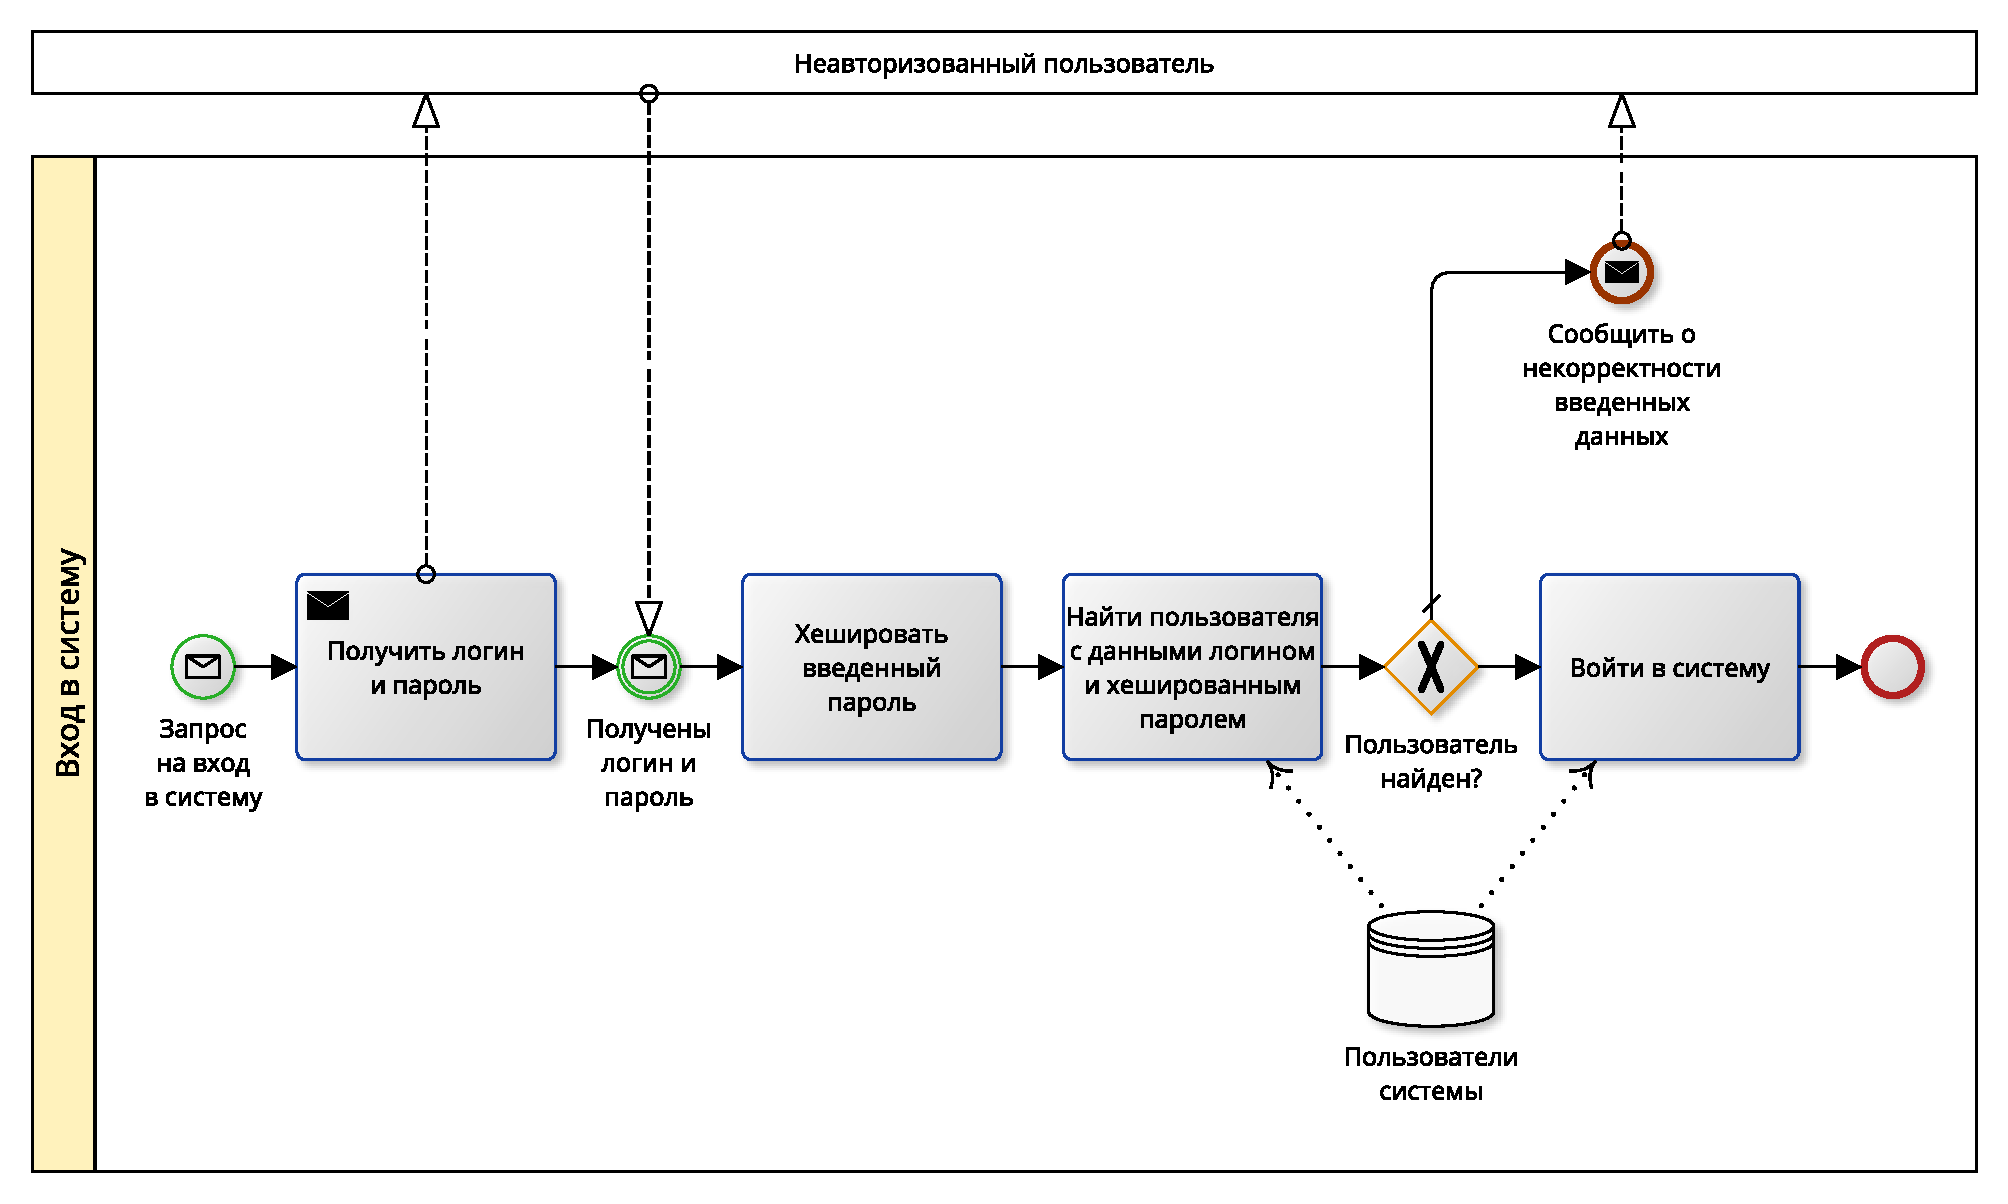
\includegraphics[width=0.8\linewidth]{bpmn_signin}
	\caption{Бизнес-правило входа в систему}
	\label{bpmn_signin}
\end{figure}
\begin{figure}[H]
	\centering
	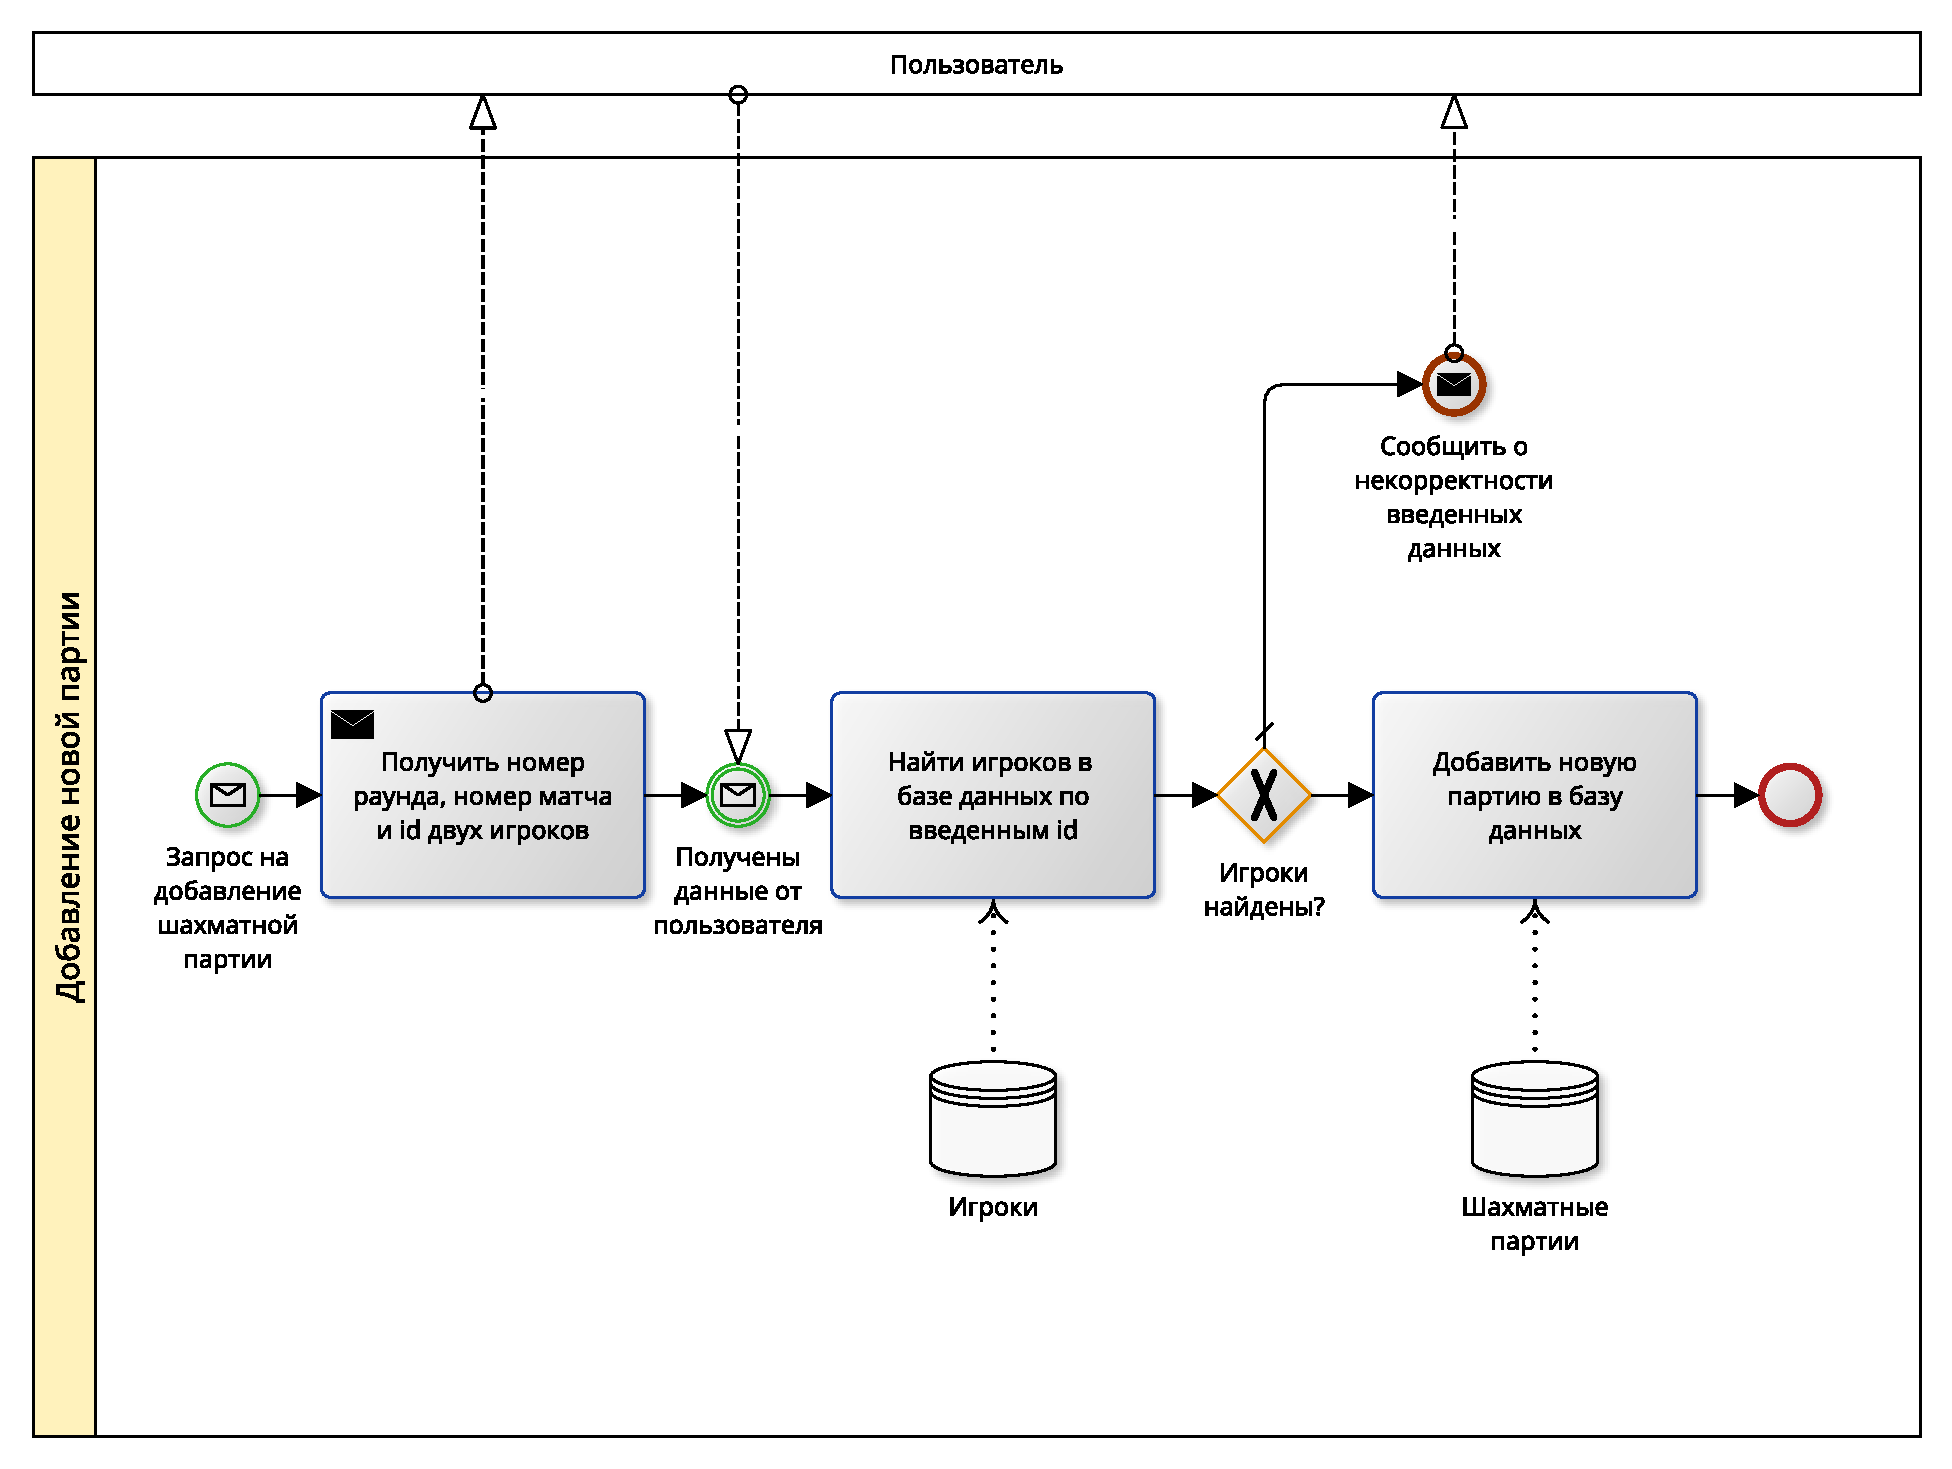
\includegraphics[width=0.8\linewidth]{bpmn_newgame}
	\caption{Бизнес-правило добавления новой шахматной партии}
	\label{bpmn_newgame}
\end{figure}
\begin{figure}[H]
	\centering
	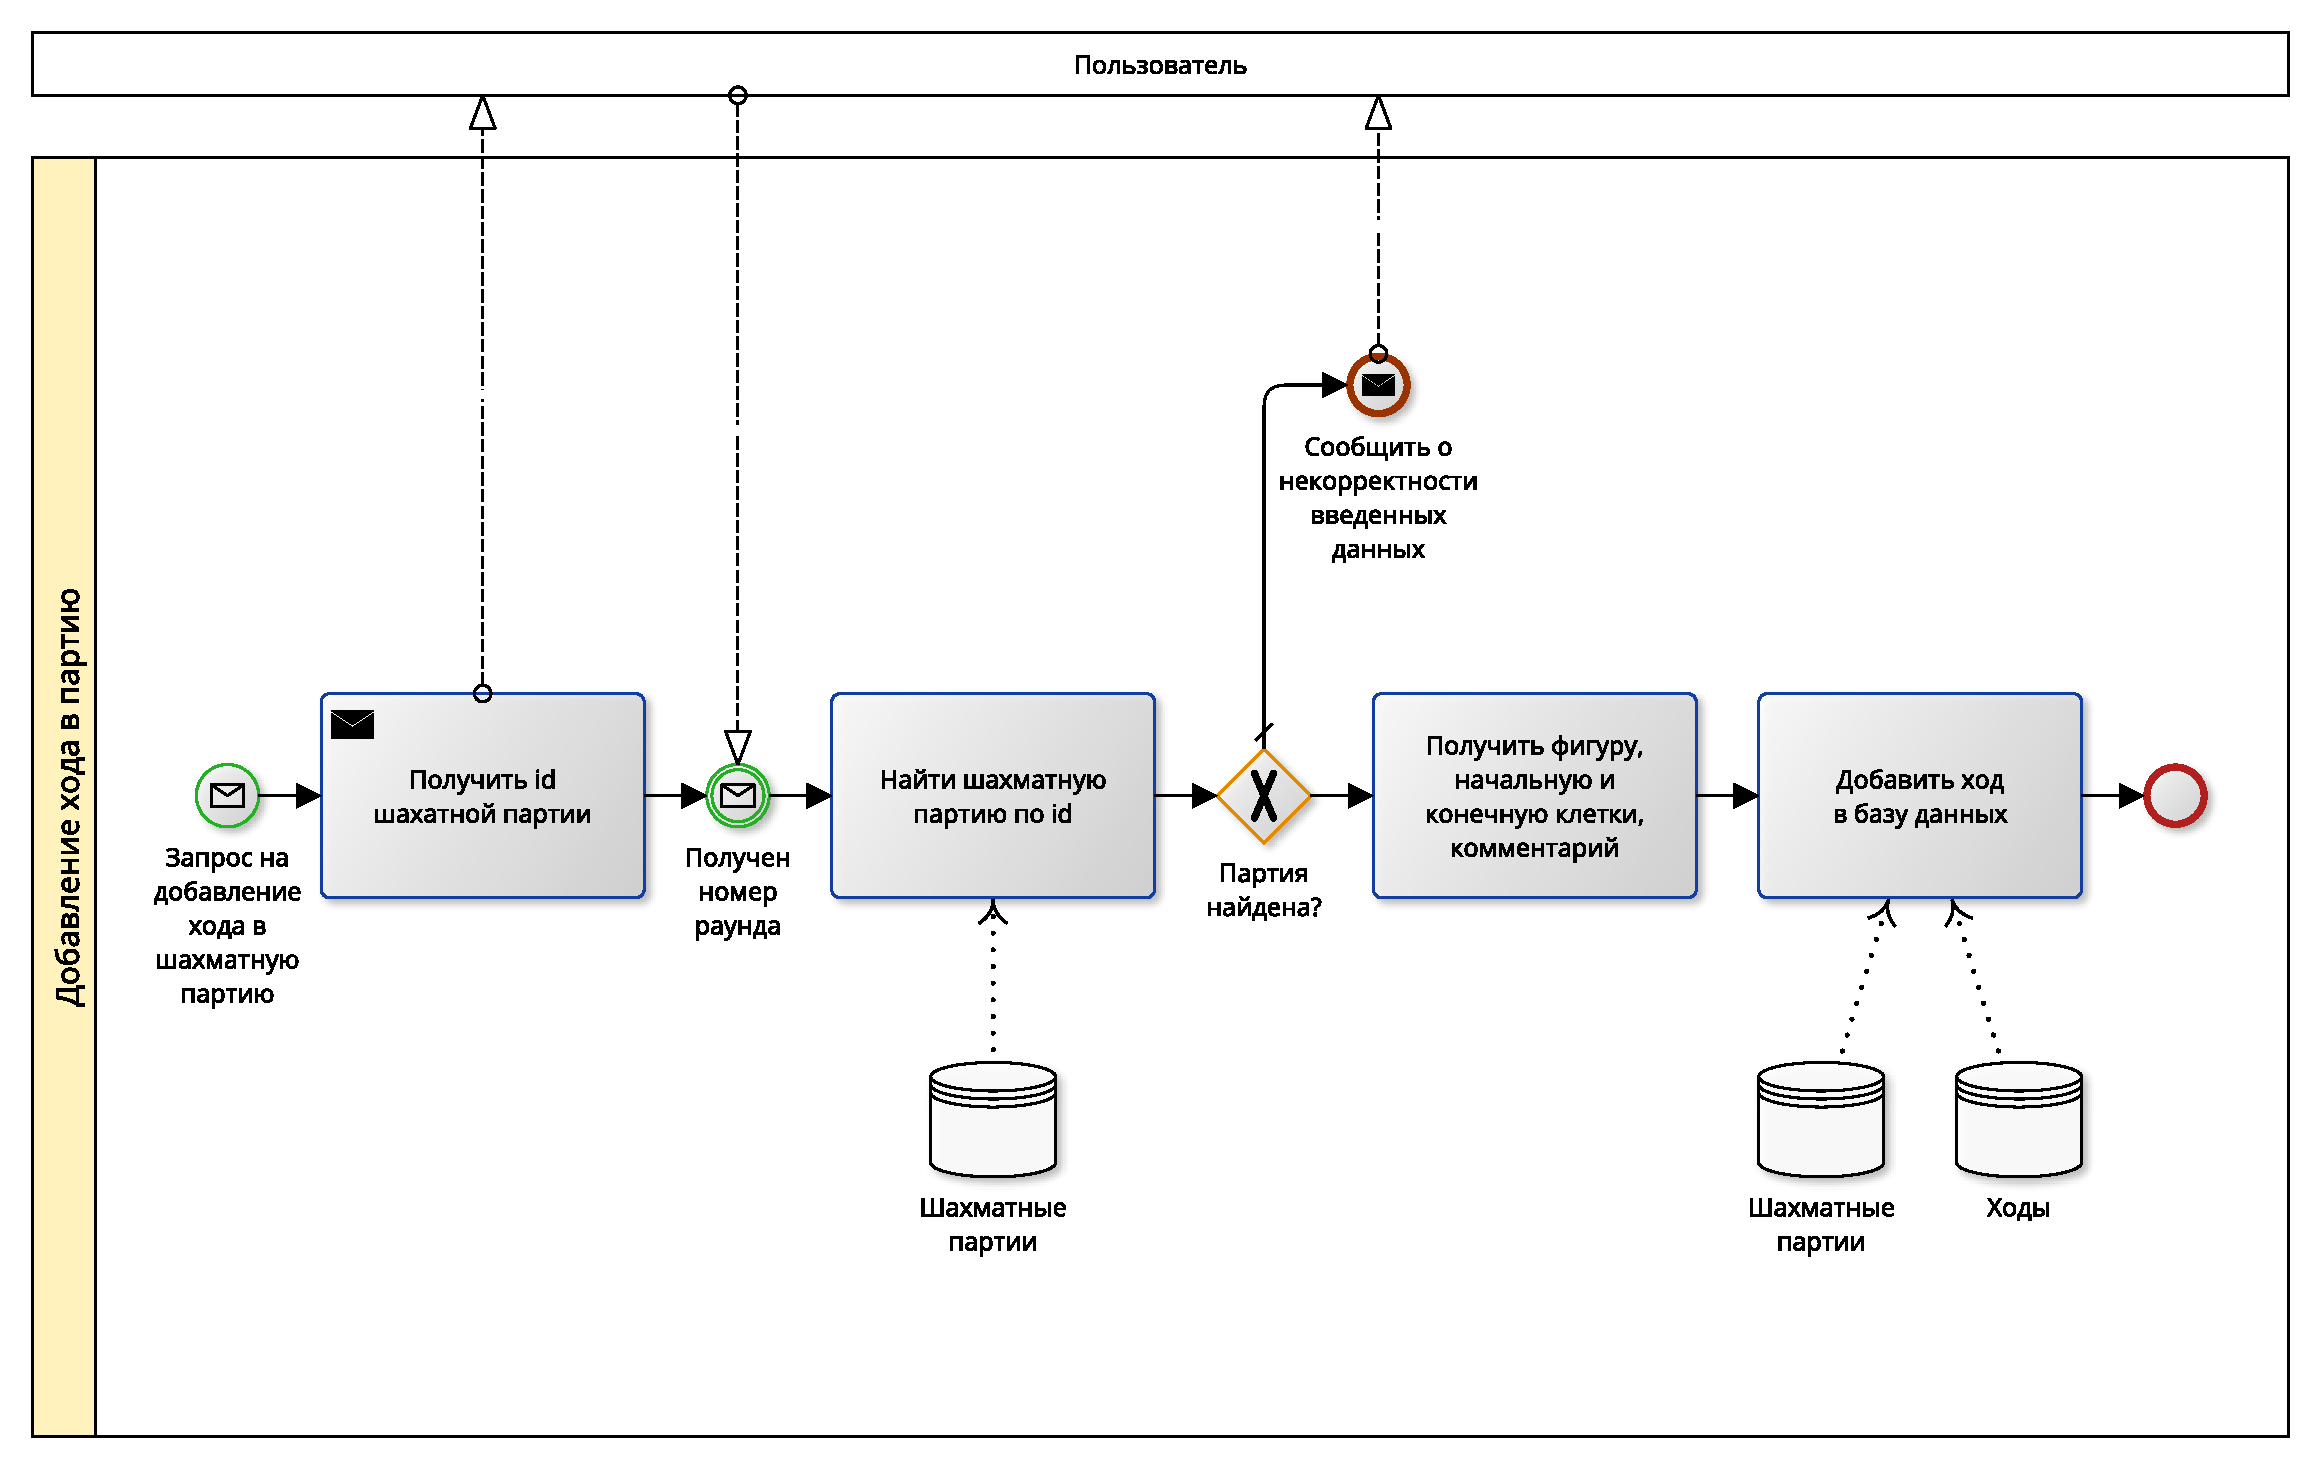
\includegraphics[width=0.8\linewidth]{bpmn_addmove}
	\caption{Бизнес-правило добавления нового хода в партию}
	\label{bpmn_addmove}
\end{figure}
\begin{figure}[H]
	\centering
	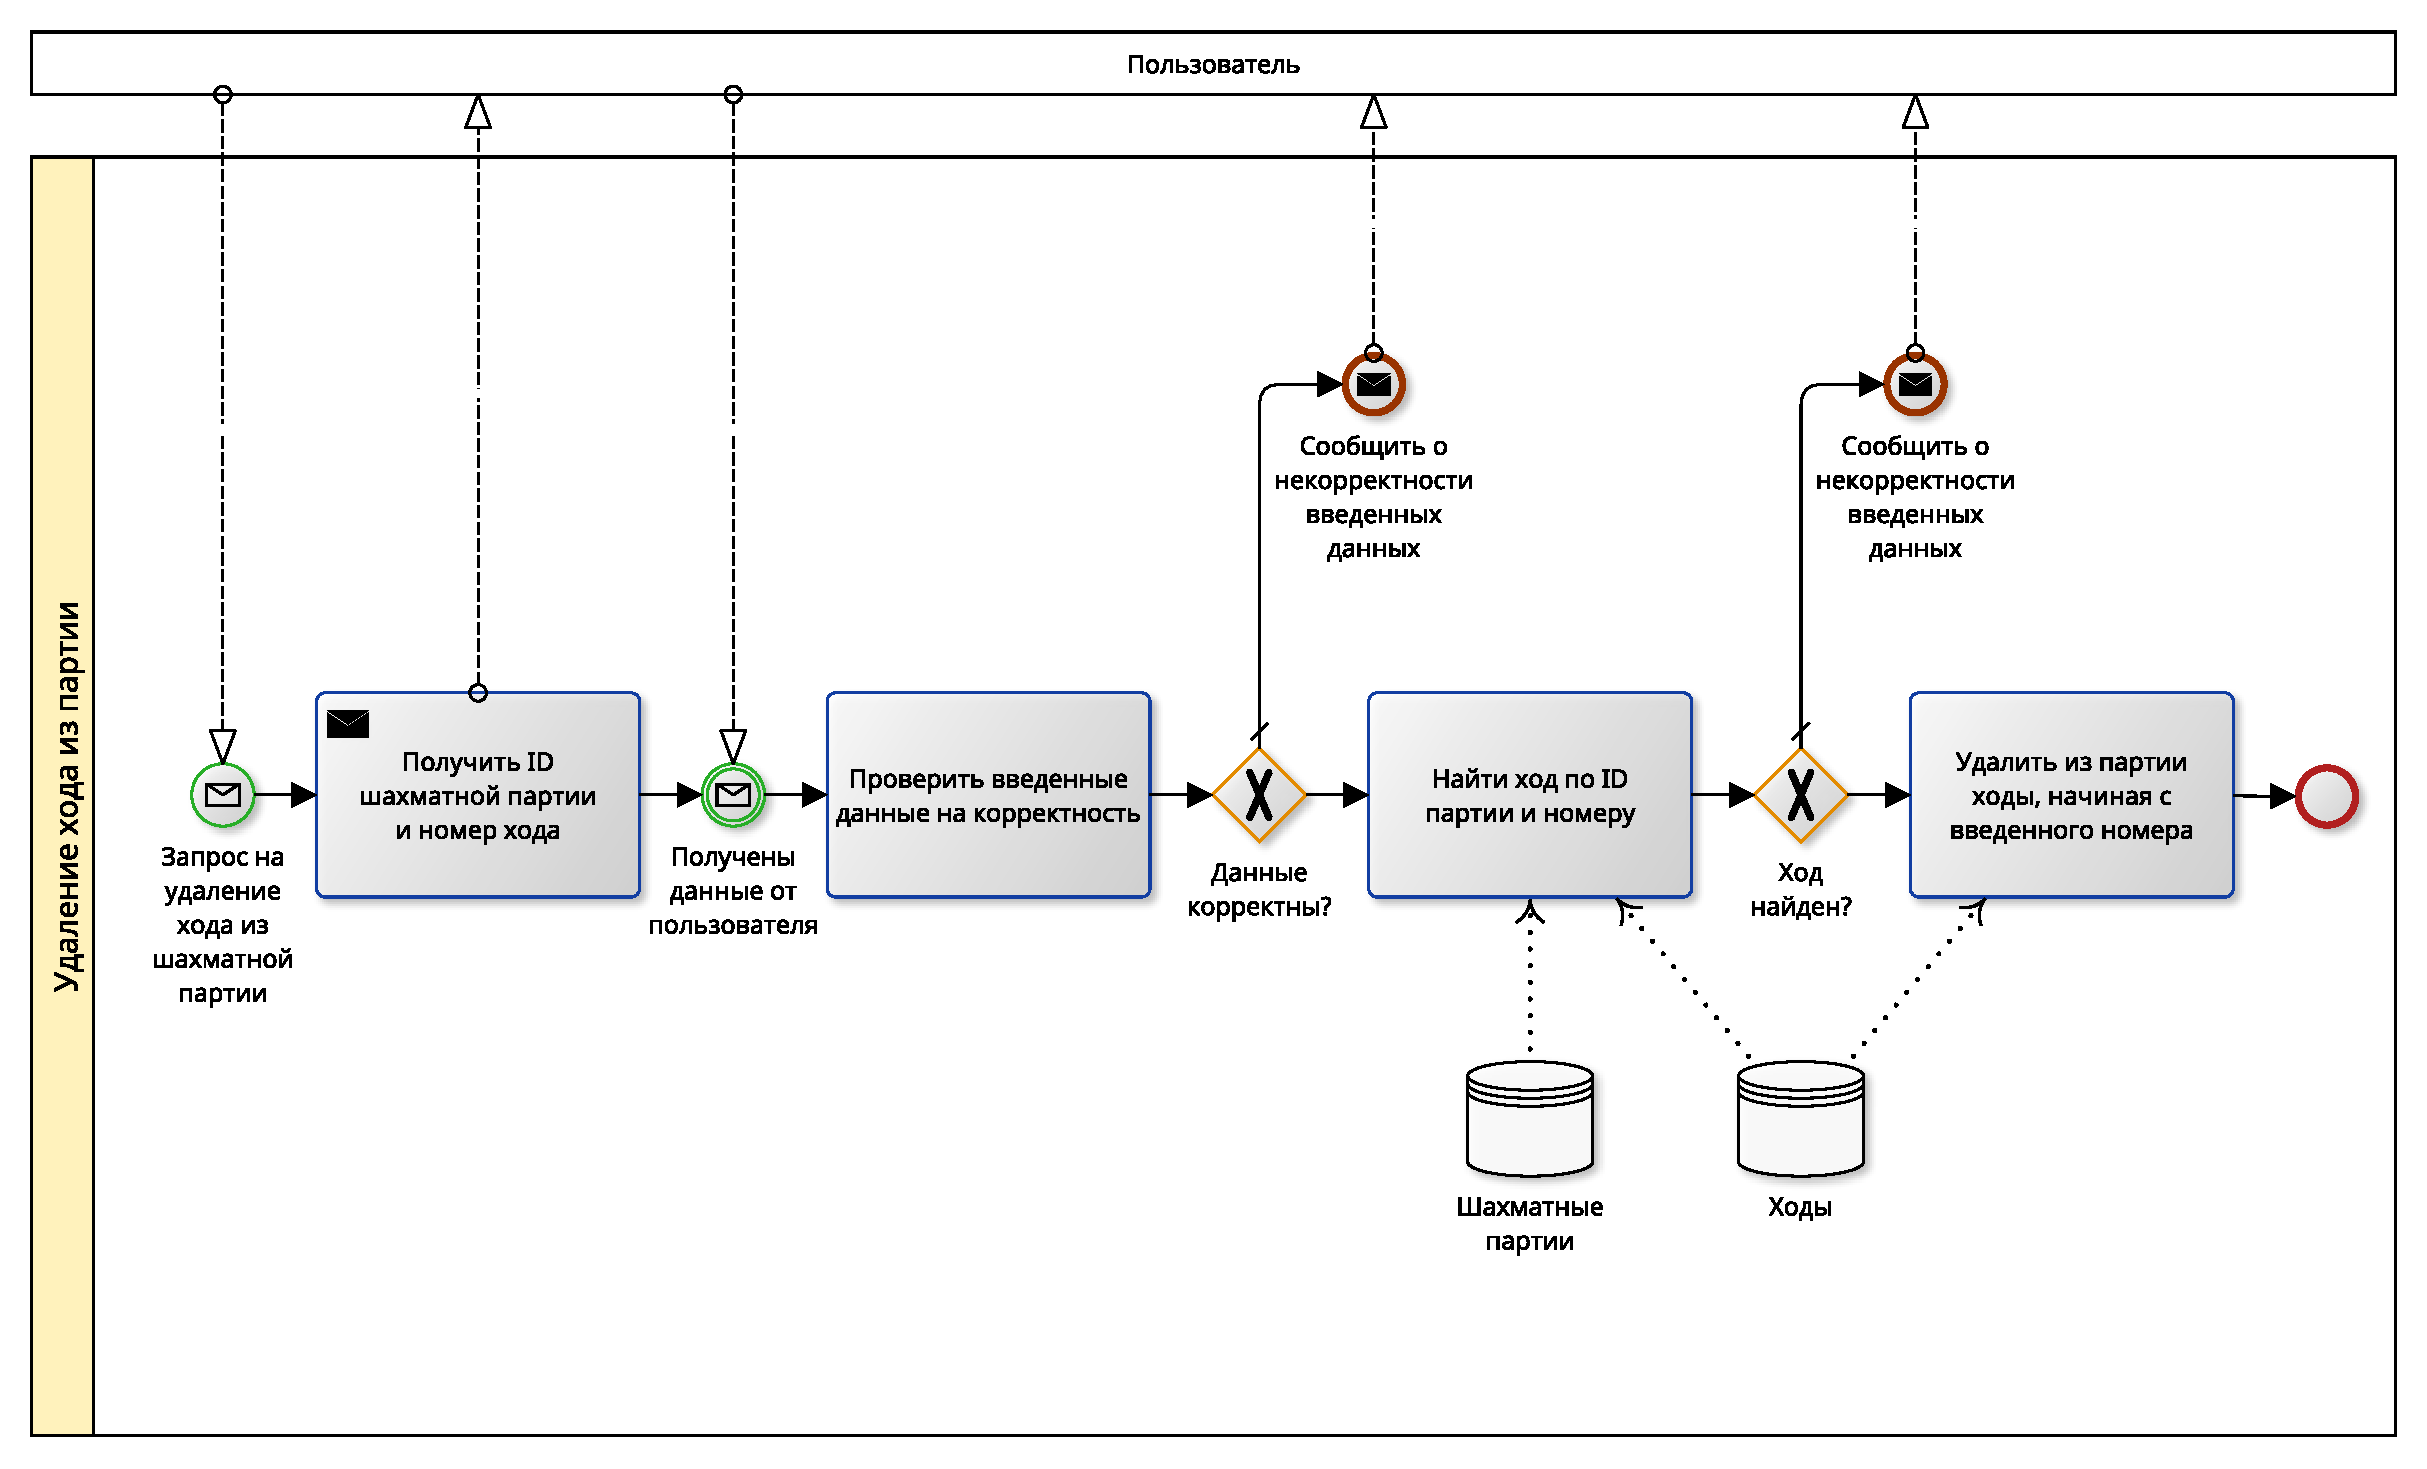
\includegraphics[width=0.8\linewidth]{bpmn_removemove}
	\caption{Бизнес-правило удаления хода из партии}
	\label{bpmn_removemove}
\end{figure}
\begin{figure}[H]
	\centering
	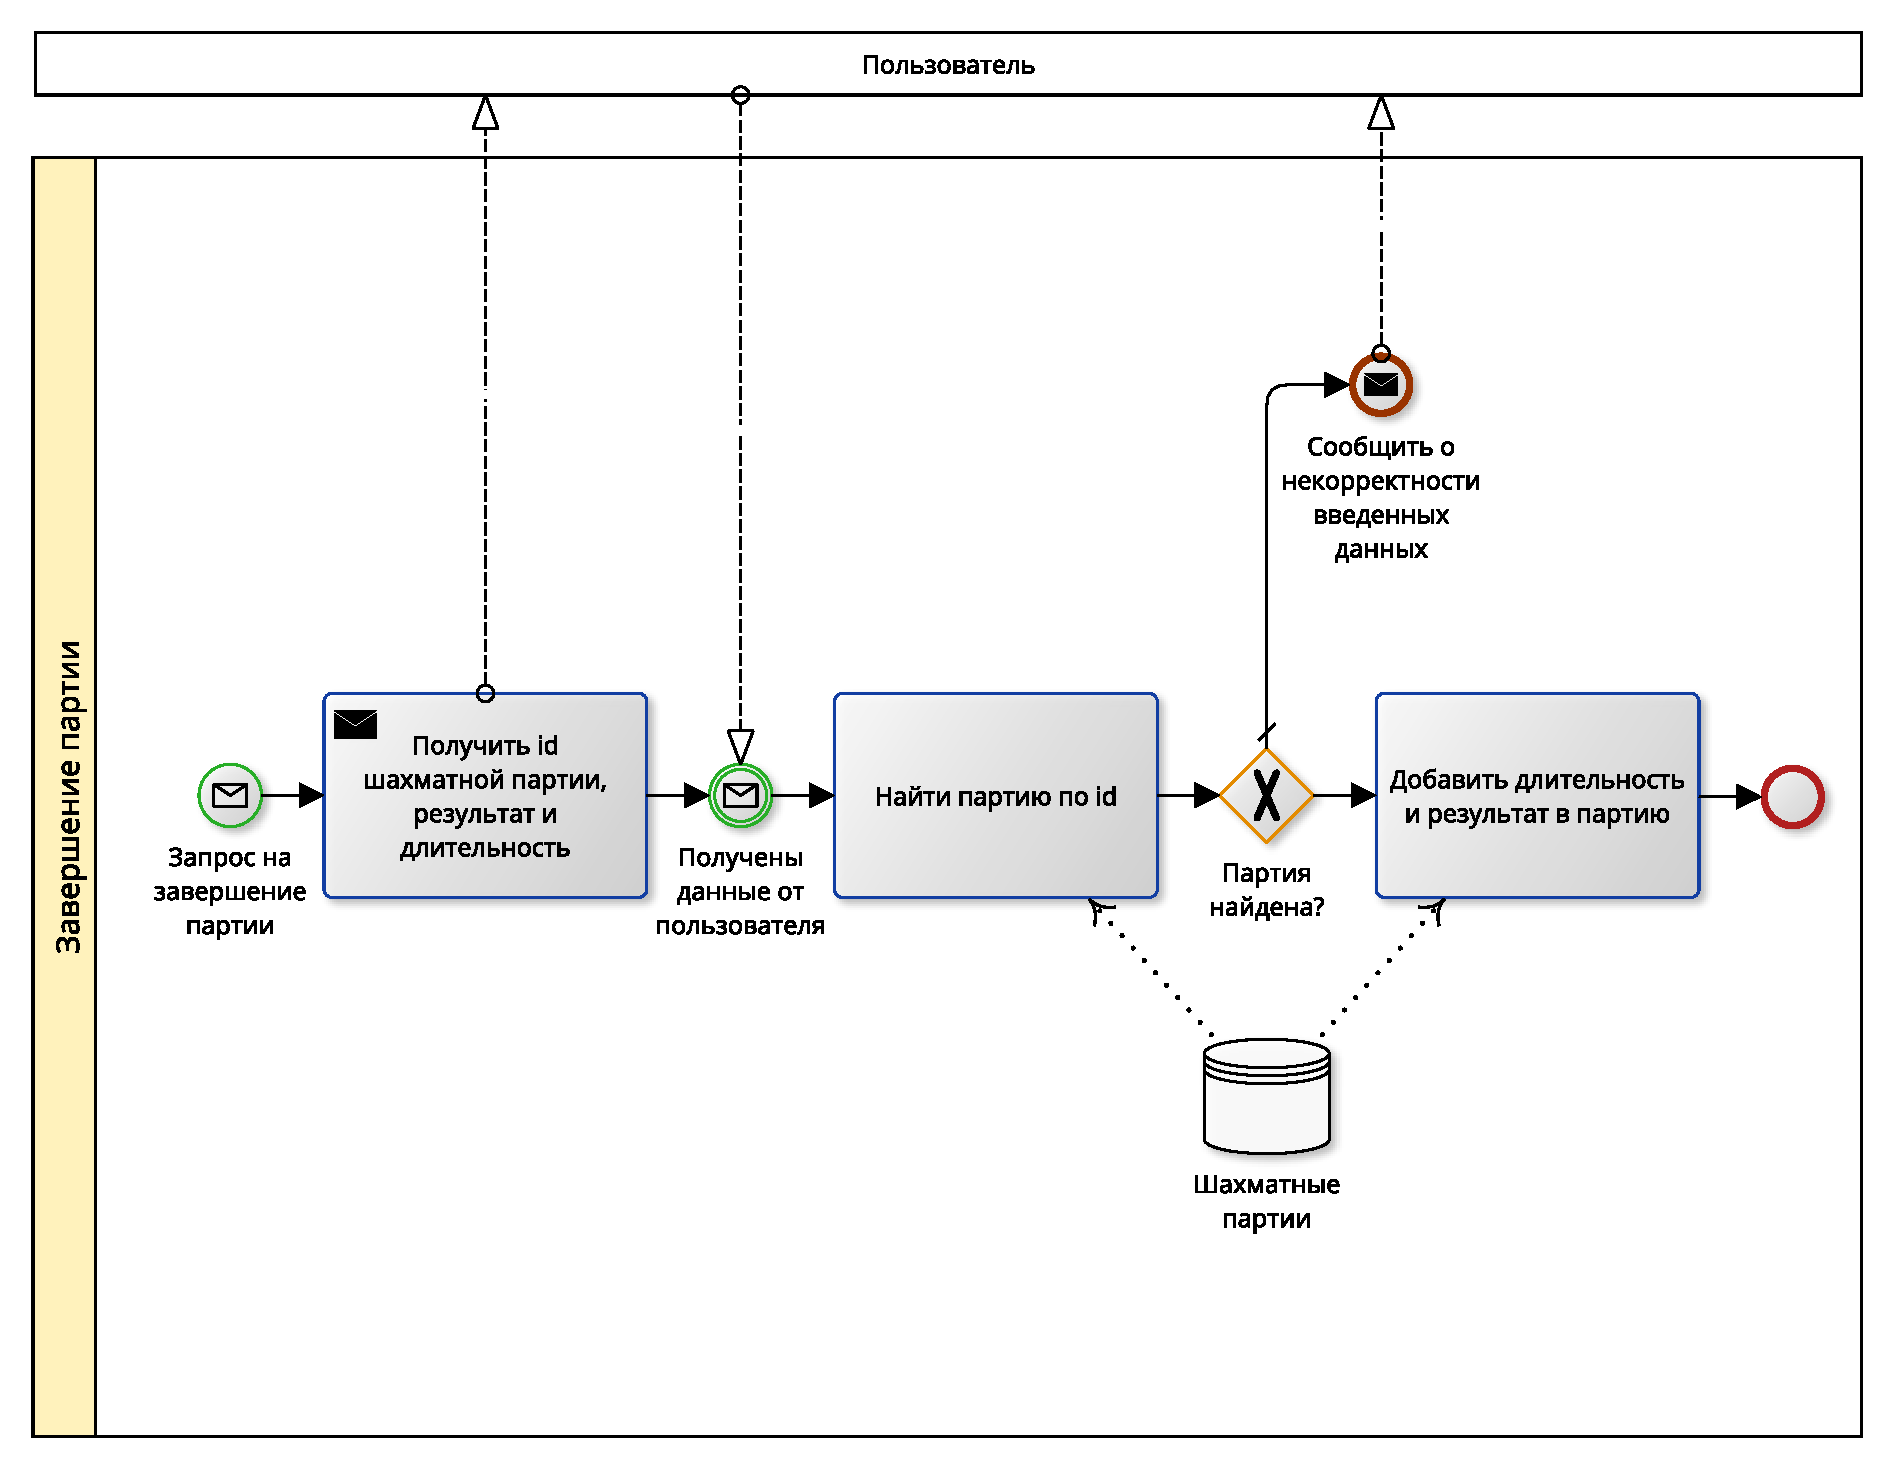
\includegraphics[width=0.8\linewidth]{bpmn_endgame}
	\caption{Бизнес-правило завершения партии}
	\label{bpmn_endgame}
\end{figure}
\begin{figure}[H]
	\centering
	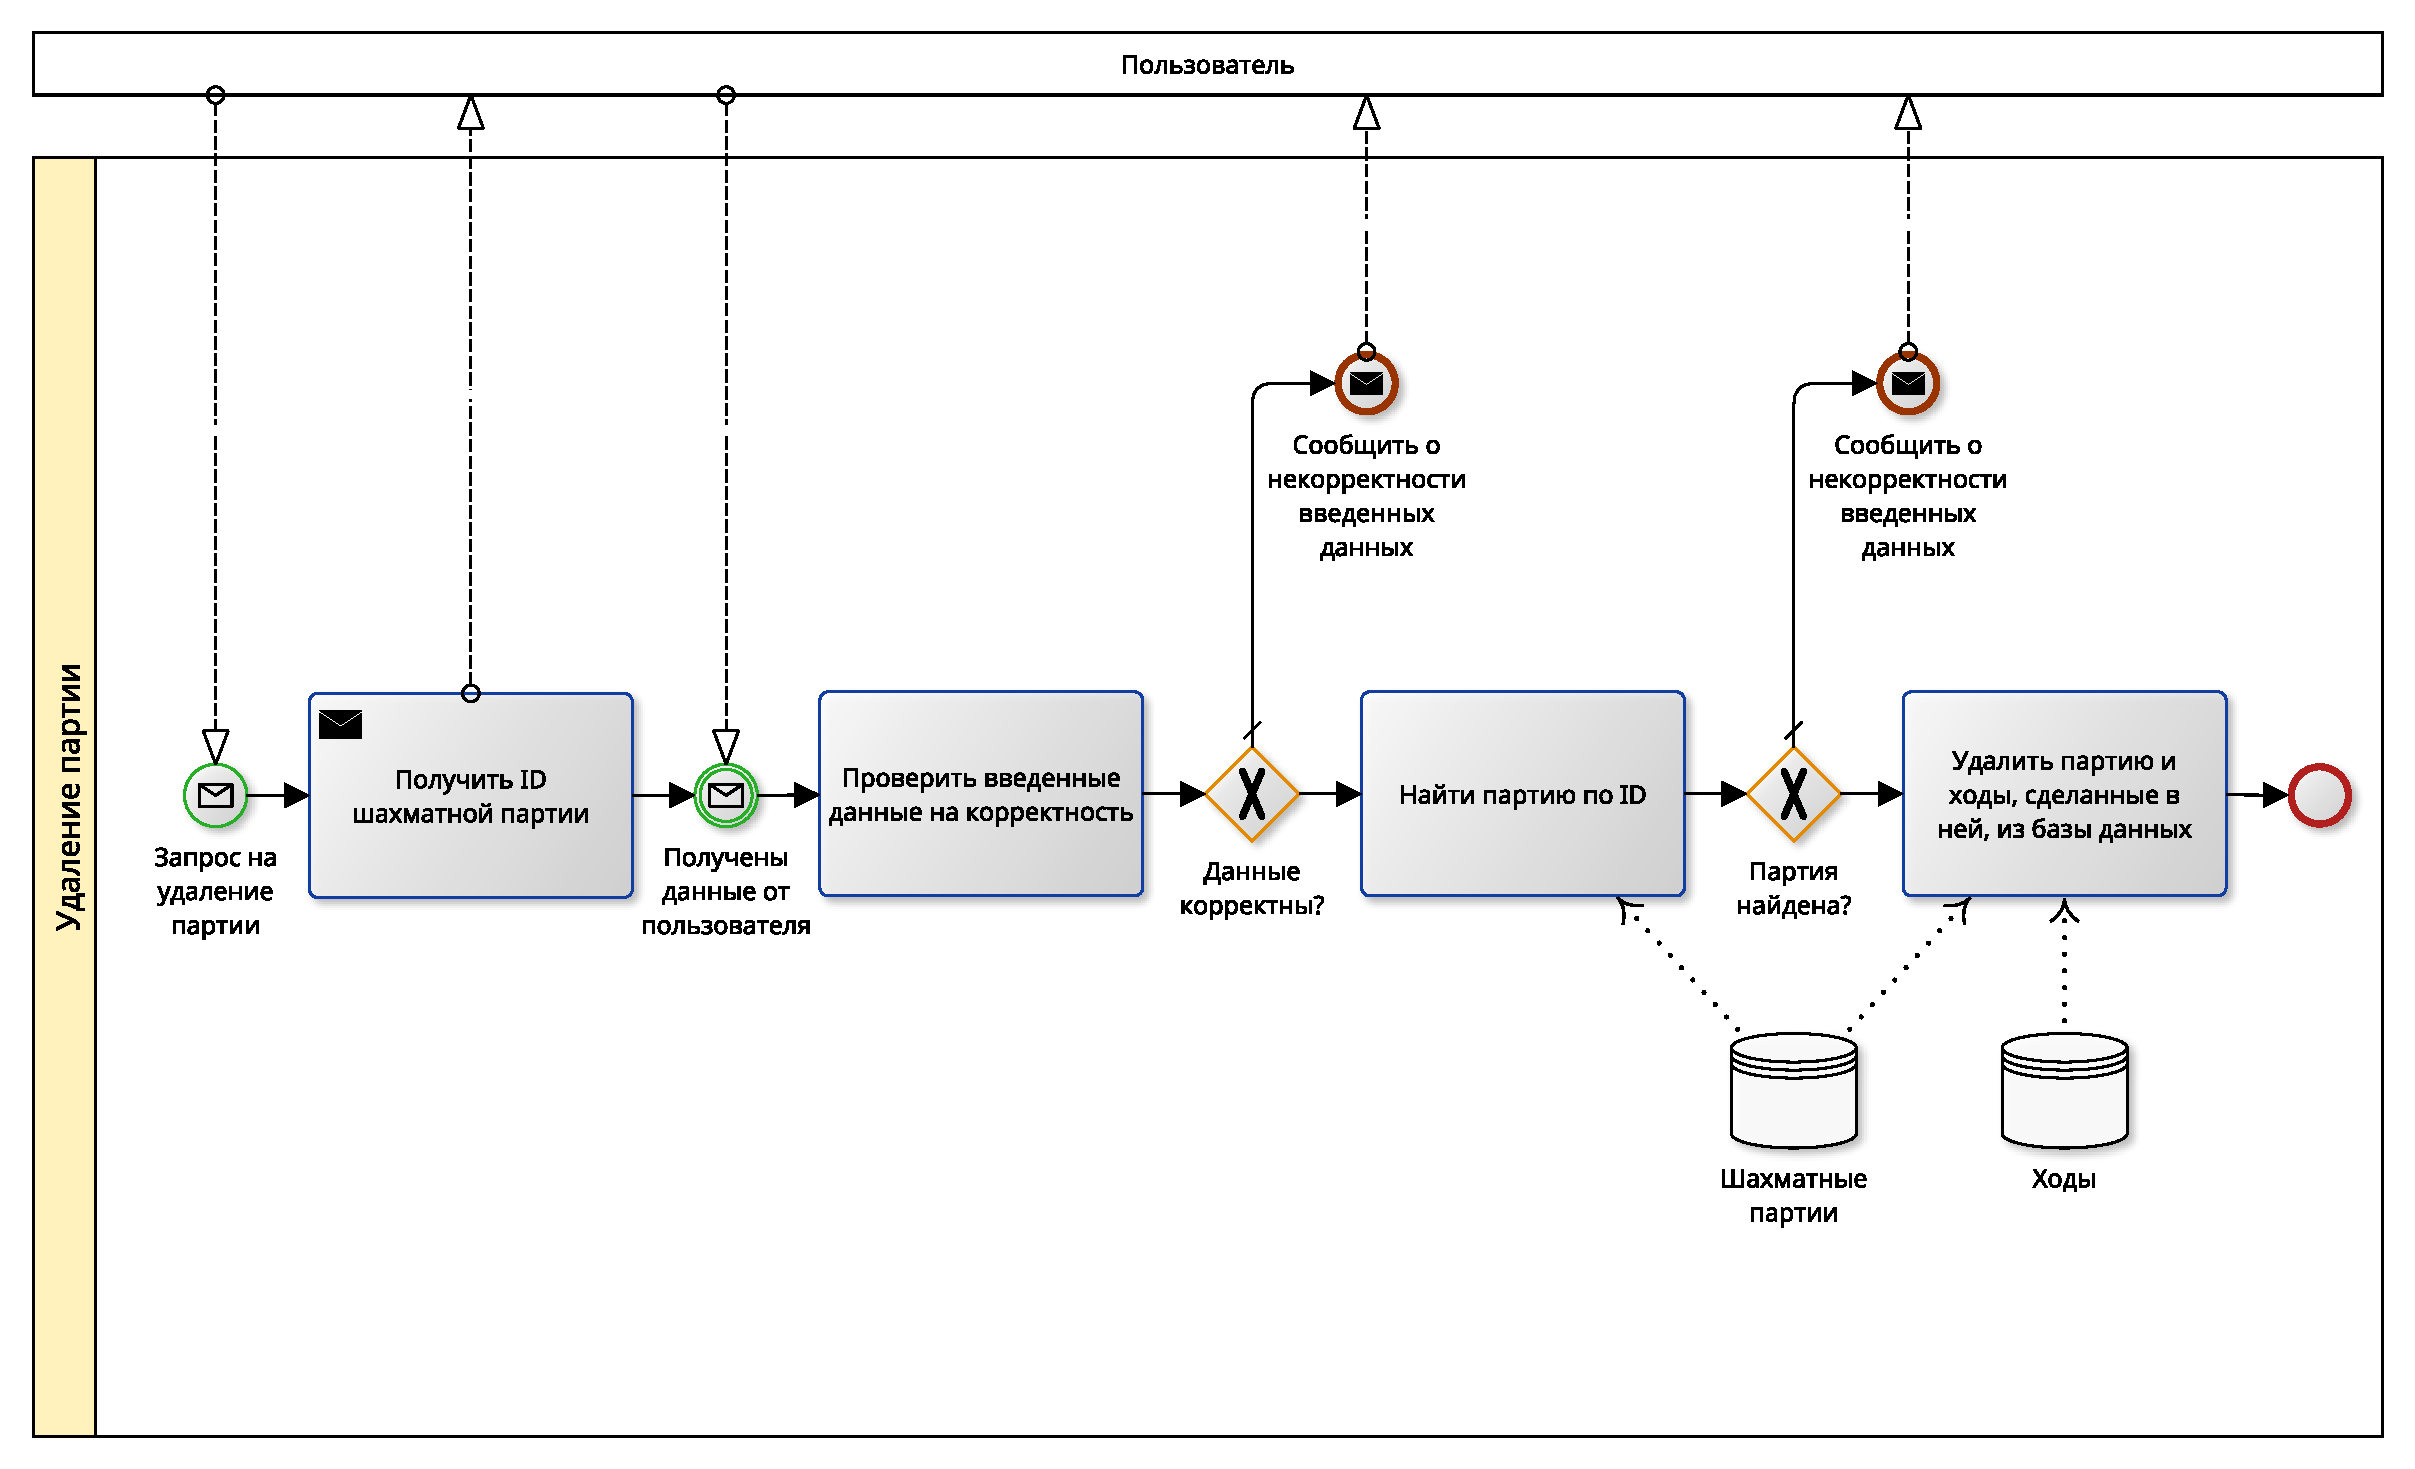
\includegraphics[width=0.8\linewidth]{bpmn_removegame}
	\caption{Бизнес-правило удаления партии}
	\label{bpmn_removegame}
\end{figure}
\begin{figure}[H]
	\centering
	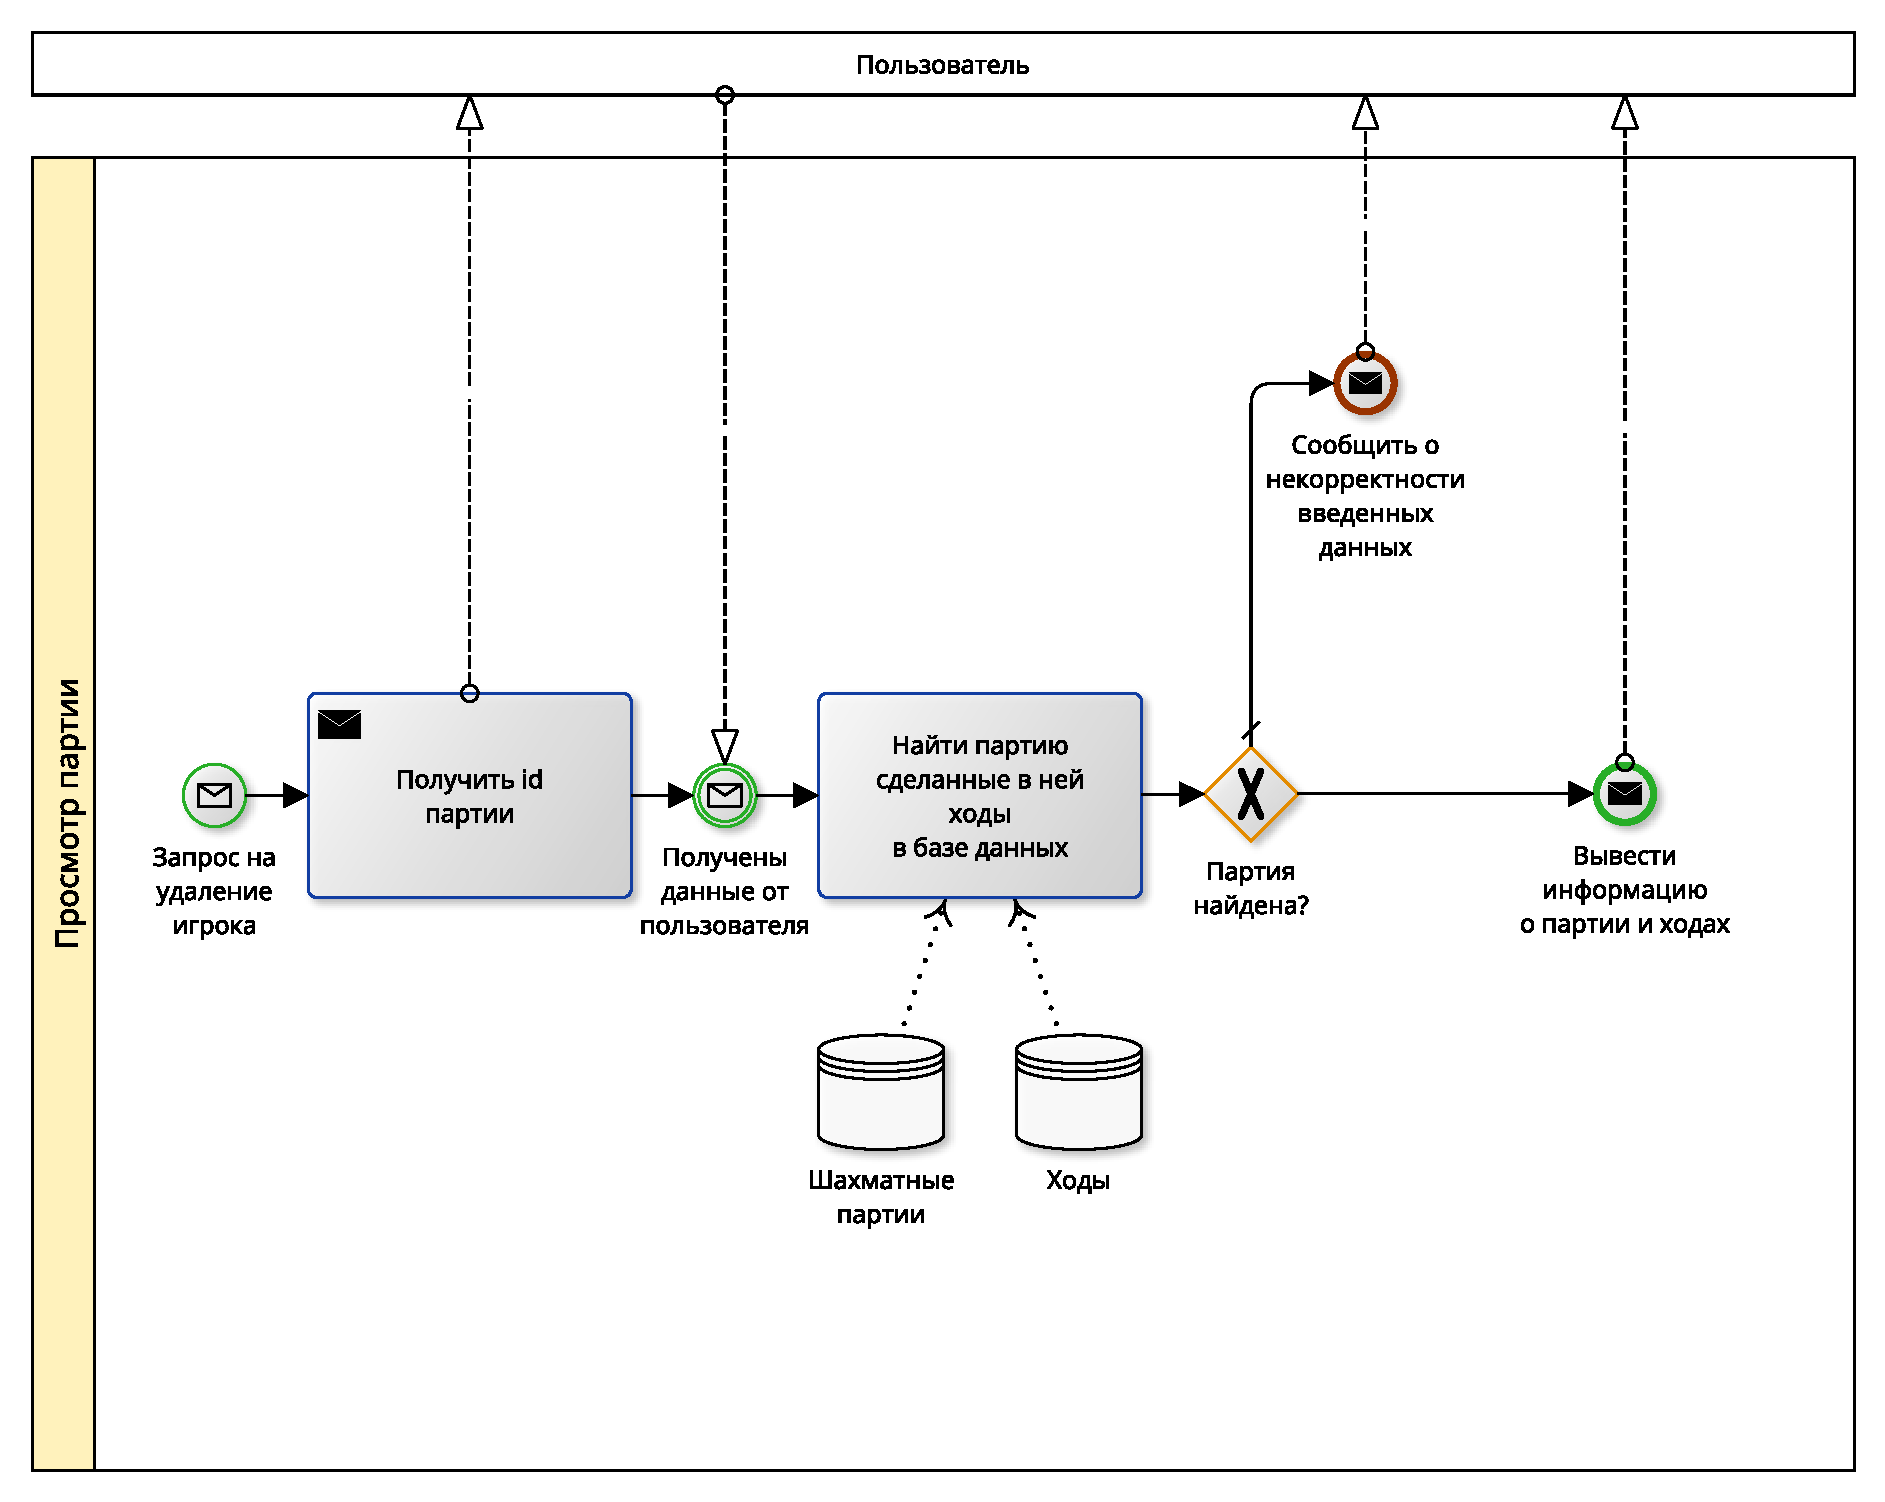
\includegraphics[width=0.8\linewidth]{bpmn_showgame}
	\caption{Бизнес-правило просмотра партии}
	\label{bpmn_showgame}
\end{figure}
\begin{figure}[H]
	\centering
	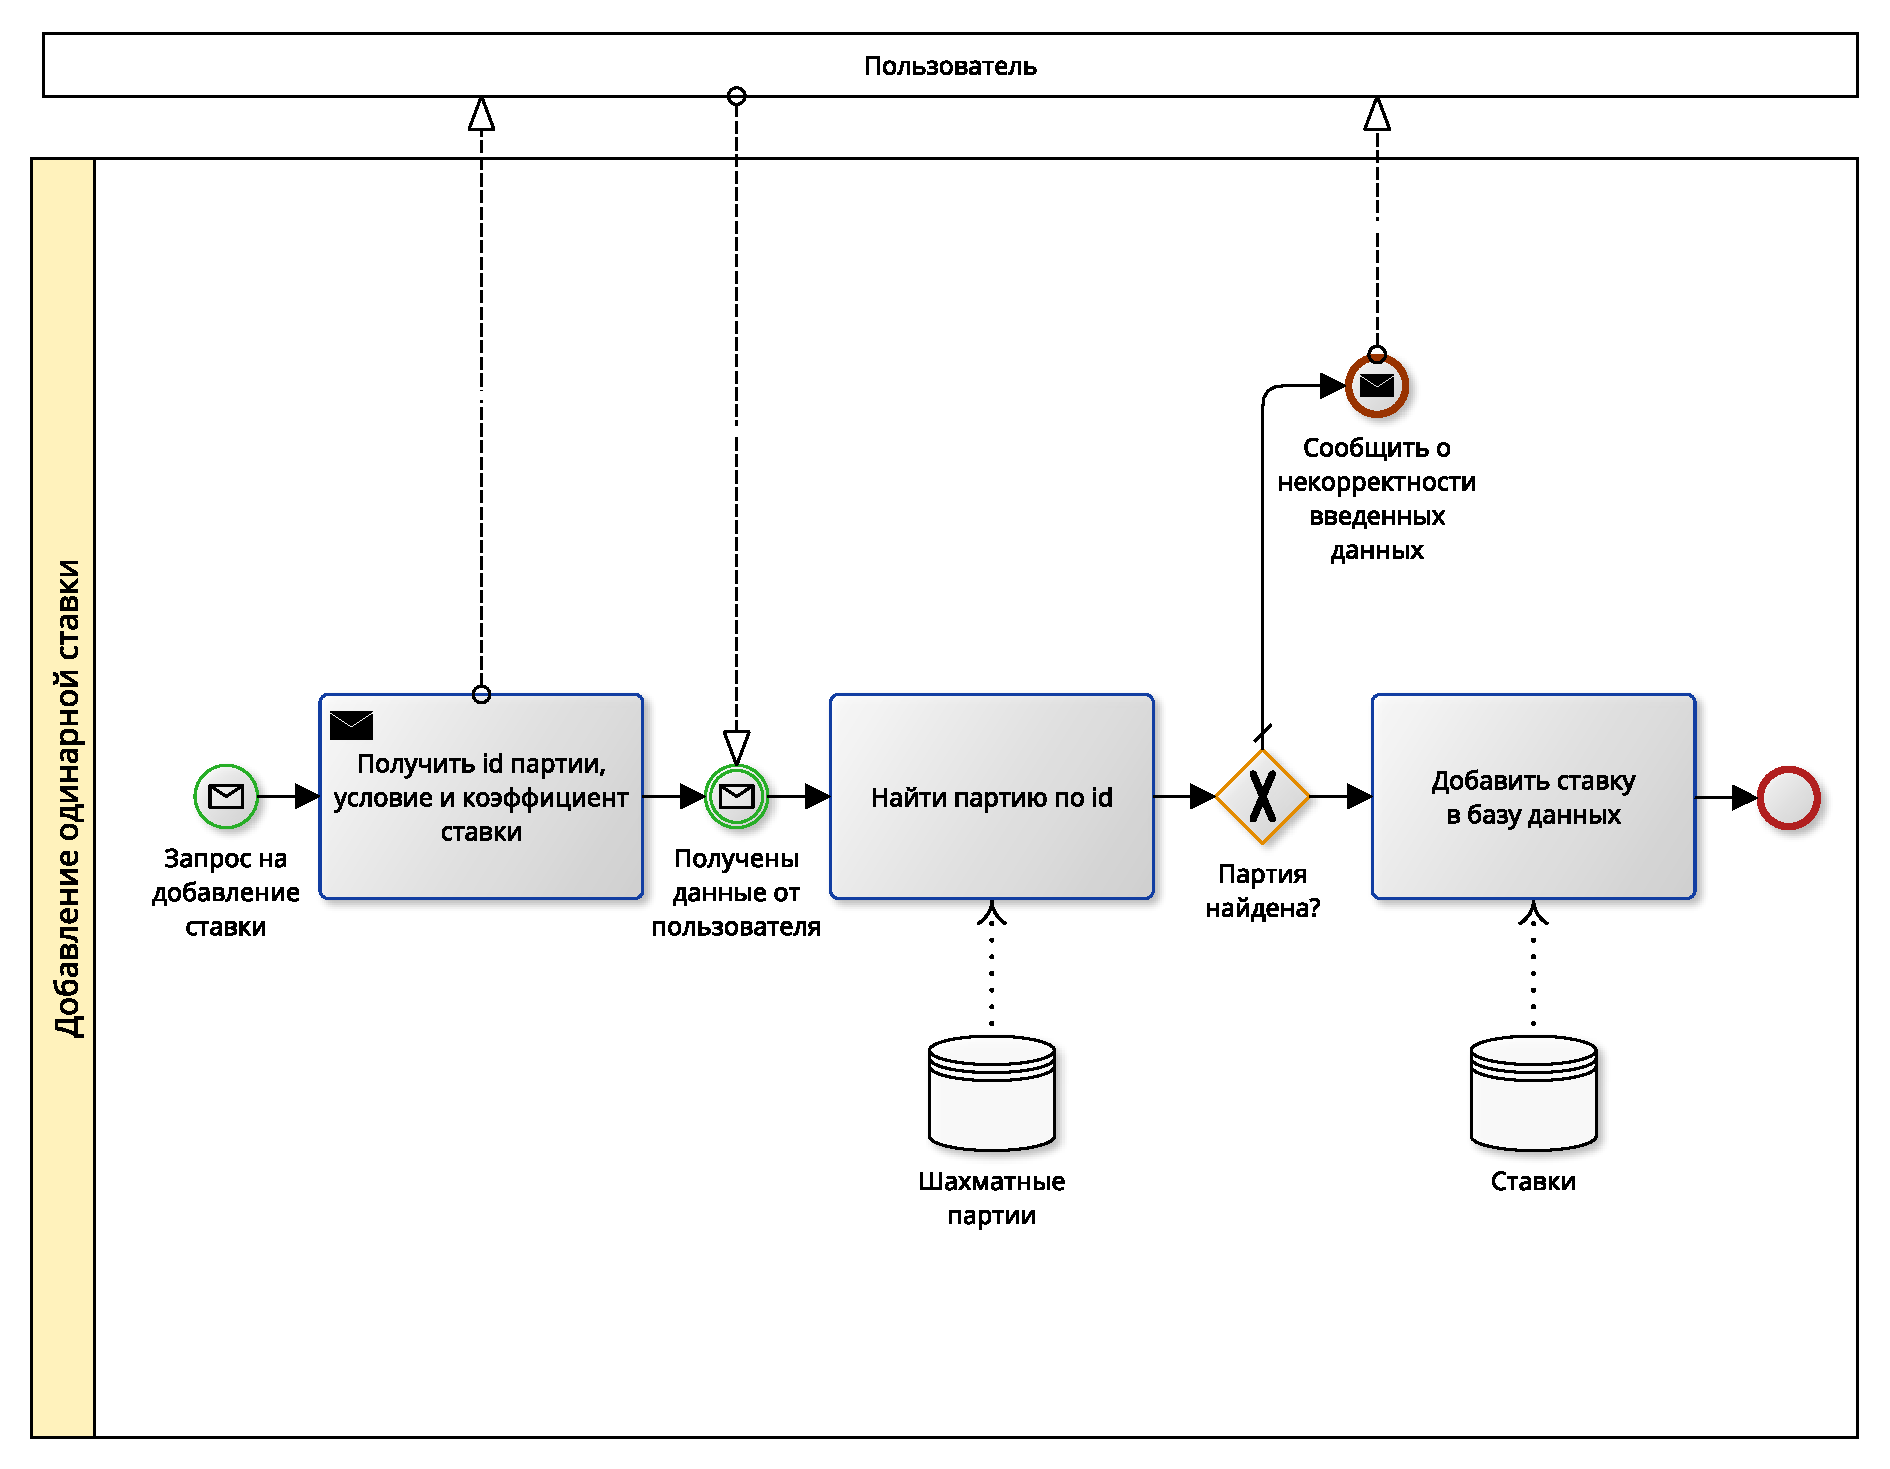
\includegraphics[width=0.8\linewidth]{bpmn_addelembet}
	\caption{Бизнес-правило добавления одинарной ставки}
	\label{bpmn_addelembet}
\end{figure}
\begin{figure}[H]
	\centering
	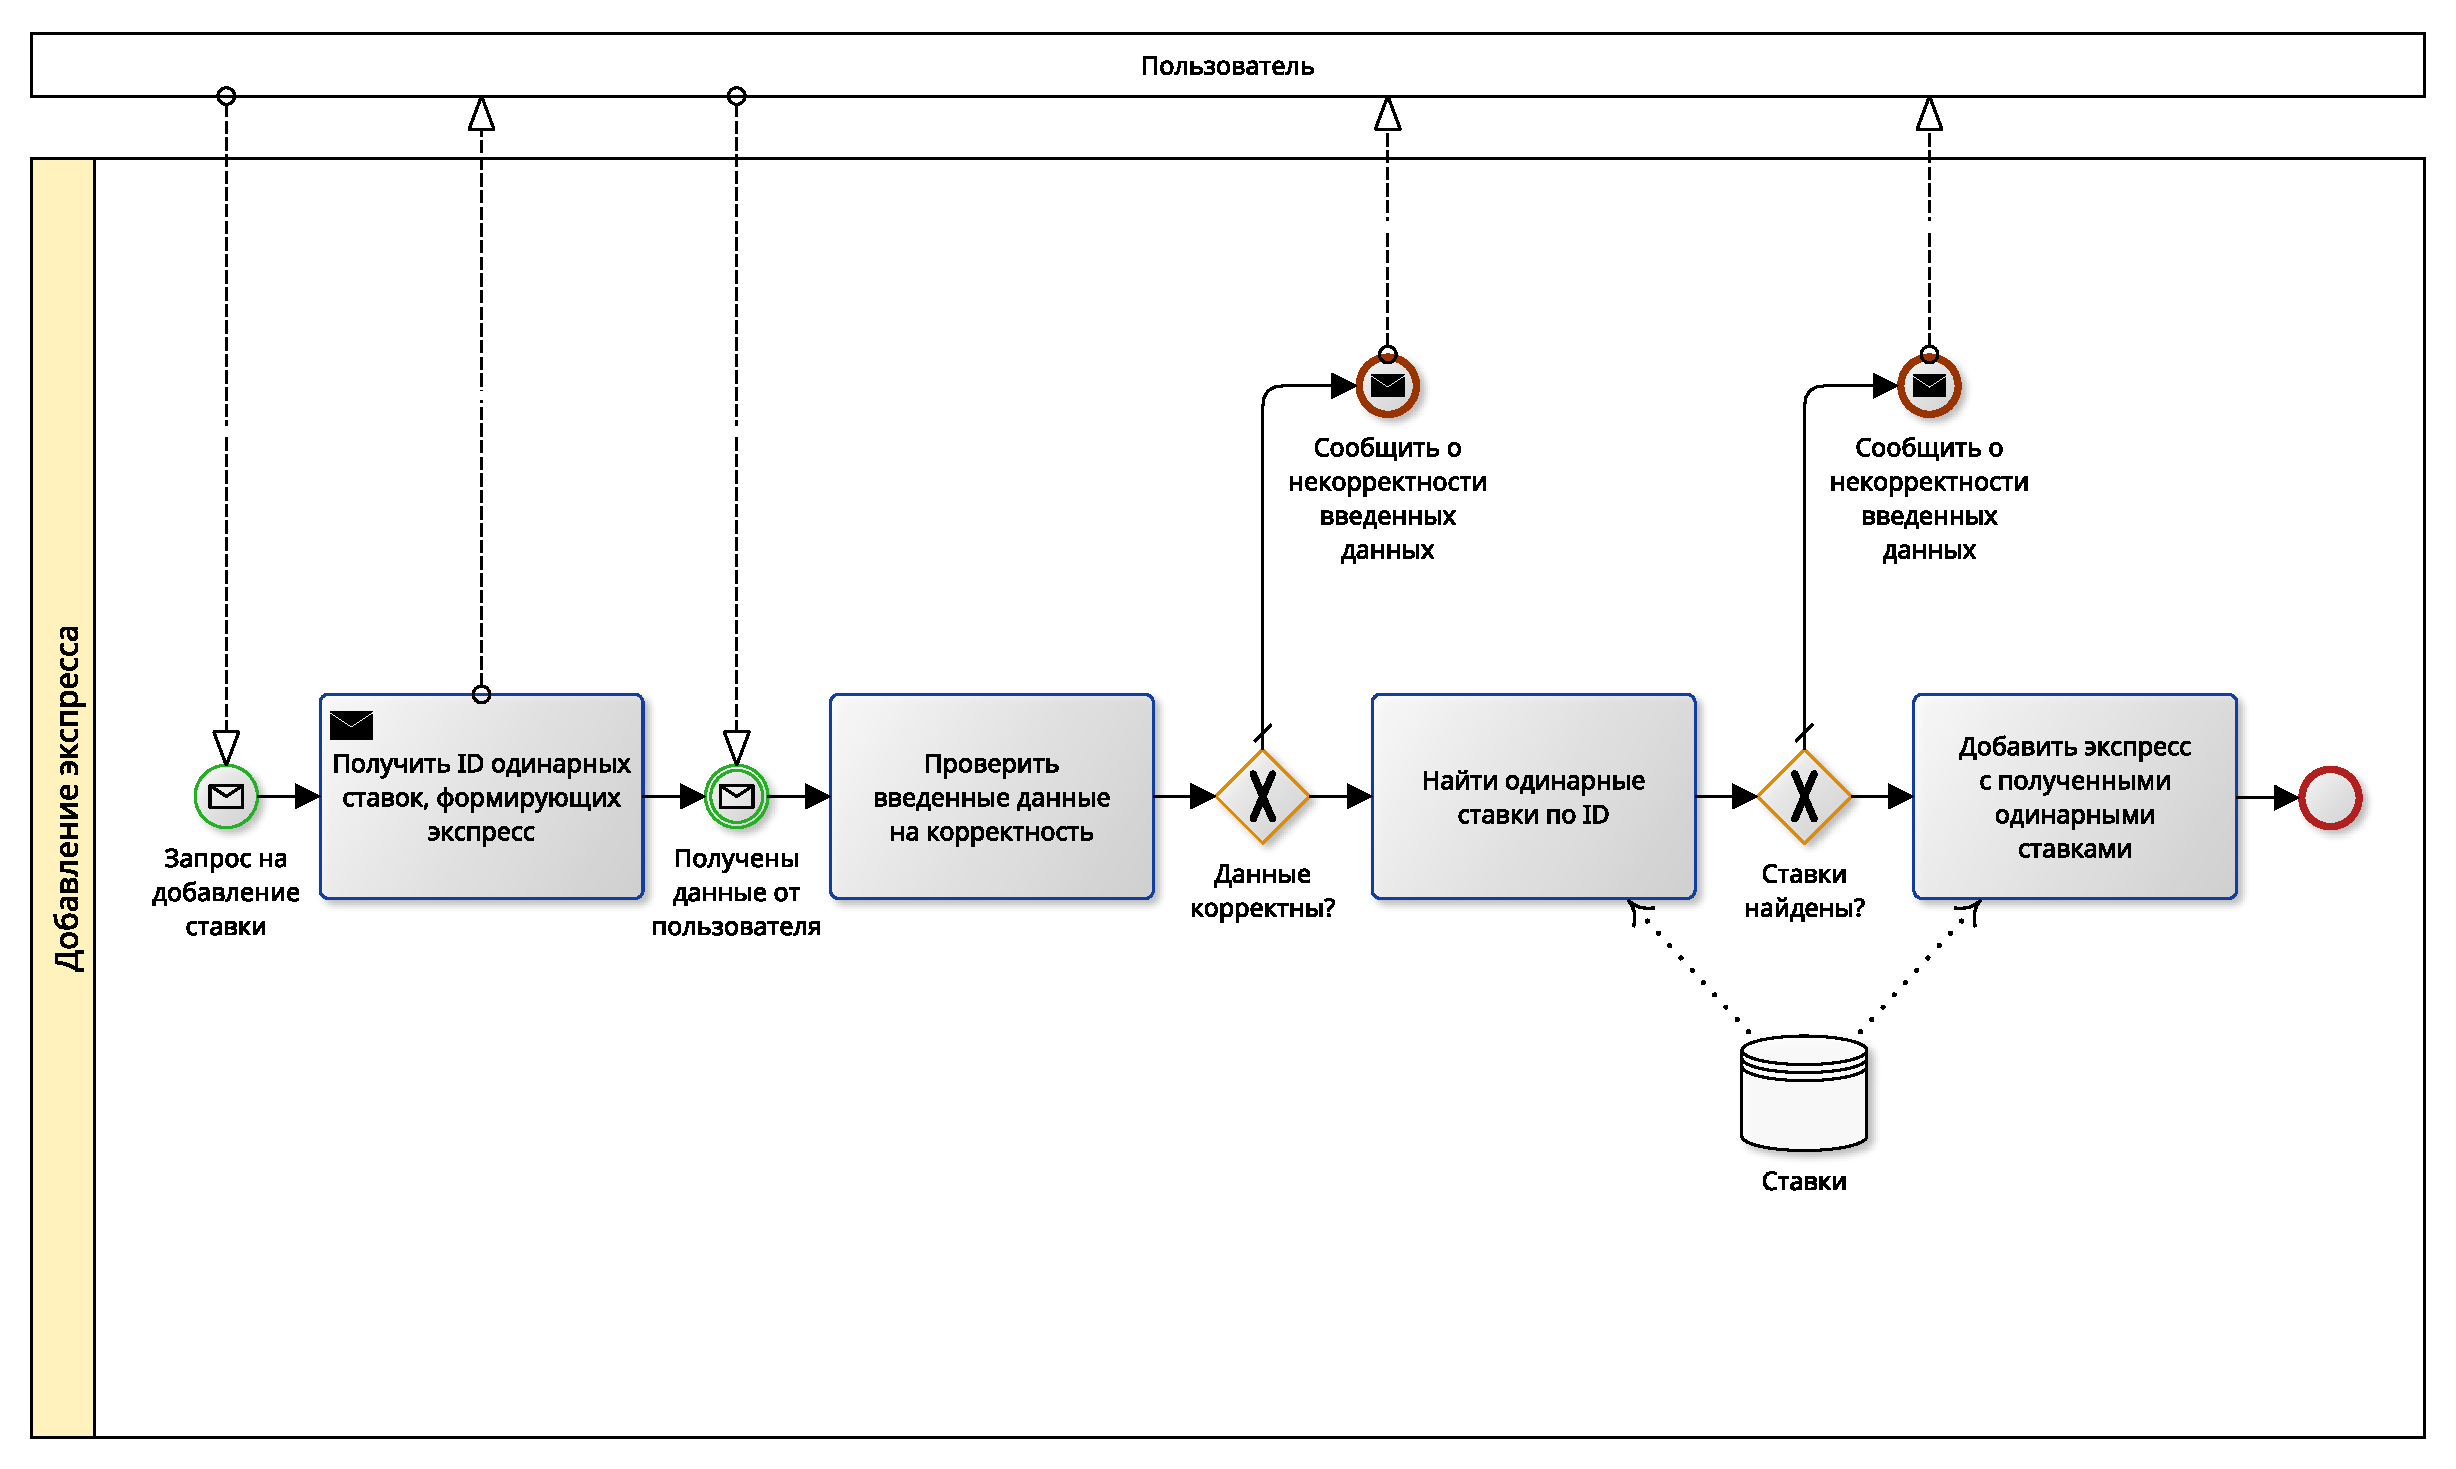
\includegraphics[width=0.6\linewidth]{bpmn_addexpress}
	\caption{Бизнес-правило добавления экспресса}
	\label{bpmn_addexpress}
\end{figure}
\begin{figure}[H]
	\centering
	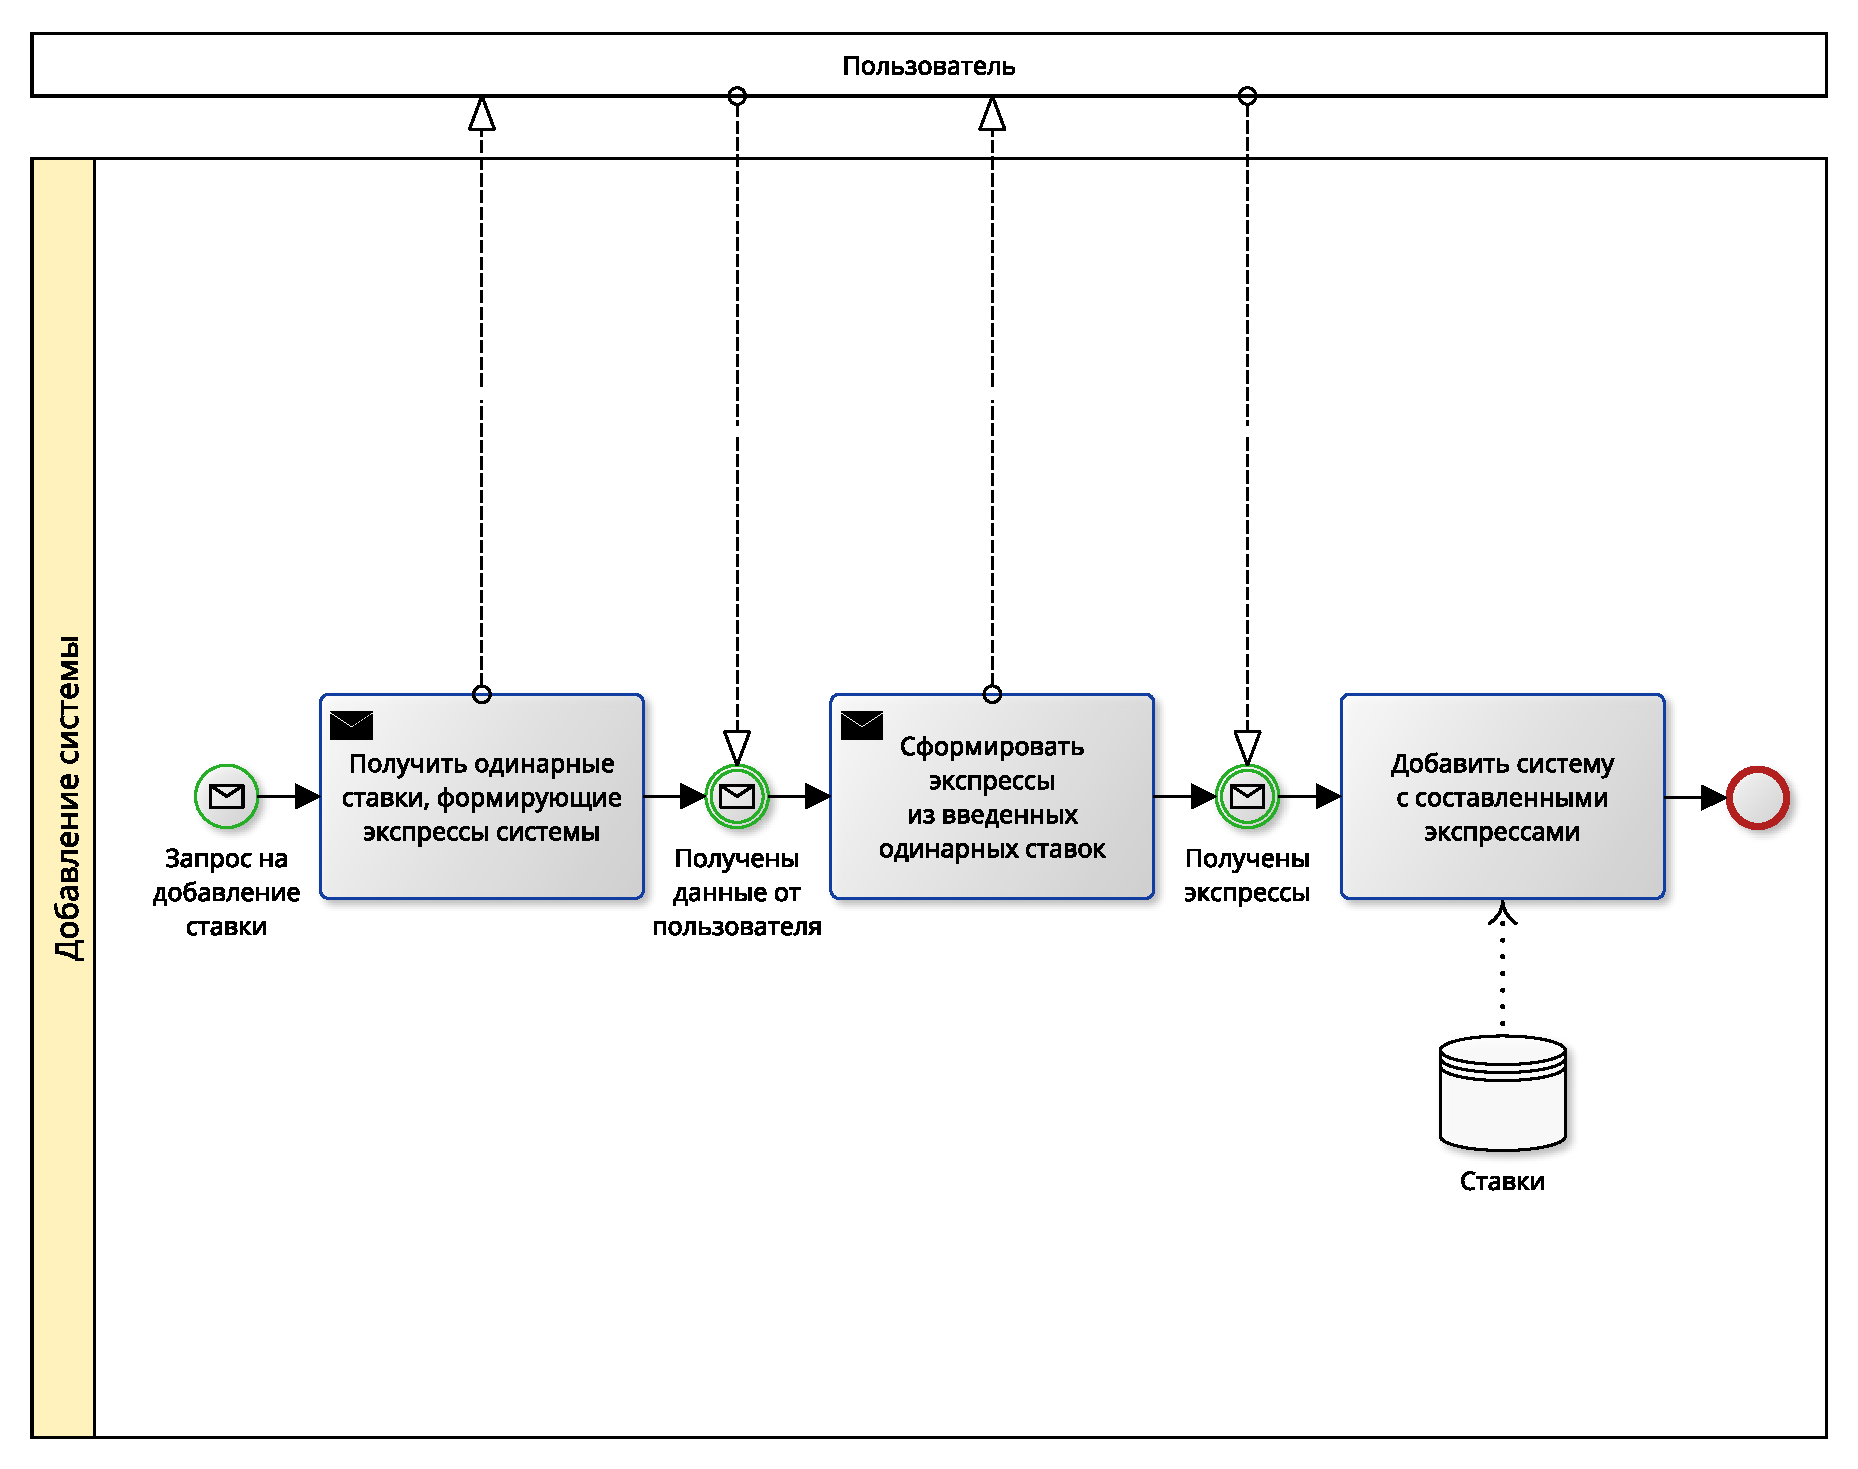
\includegraphics[width=0.8\linewidth]{bpmn_addsystem}
	\caption{Бизнес-правило добавления системы}
	\label{bpmn_addsystem}
\end{figure}
\begin{figure}[H]
	\centering
	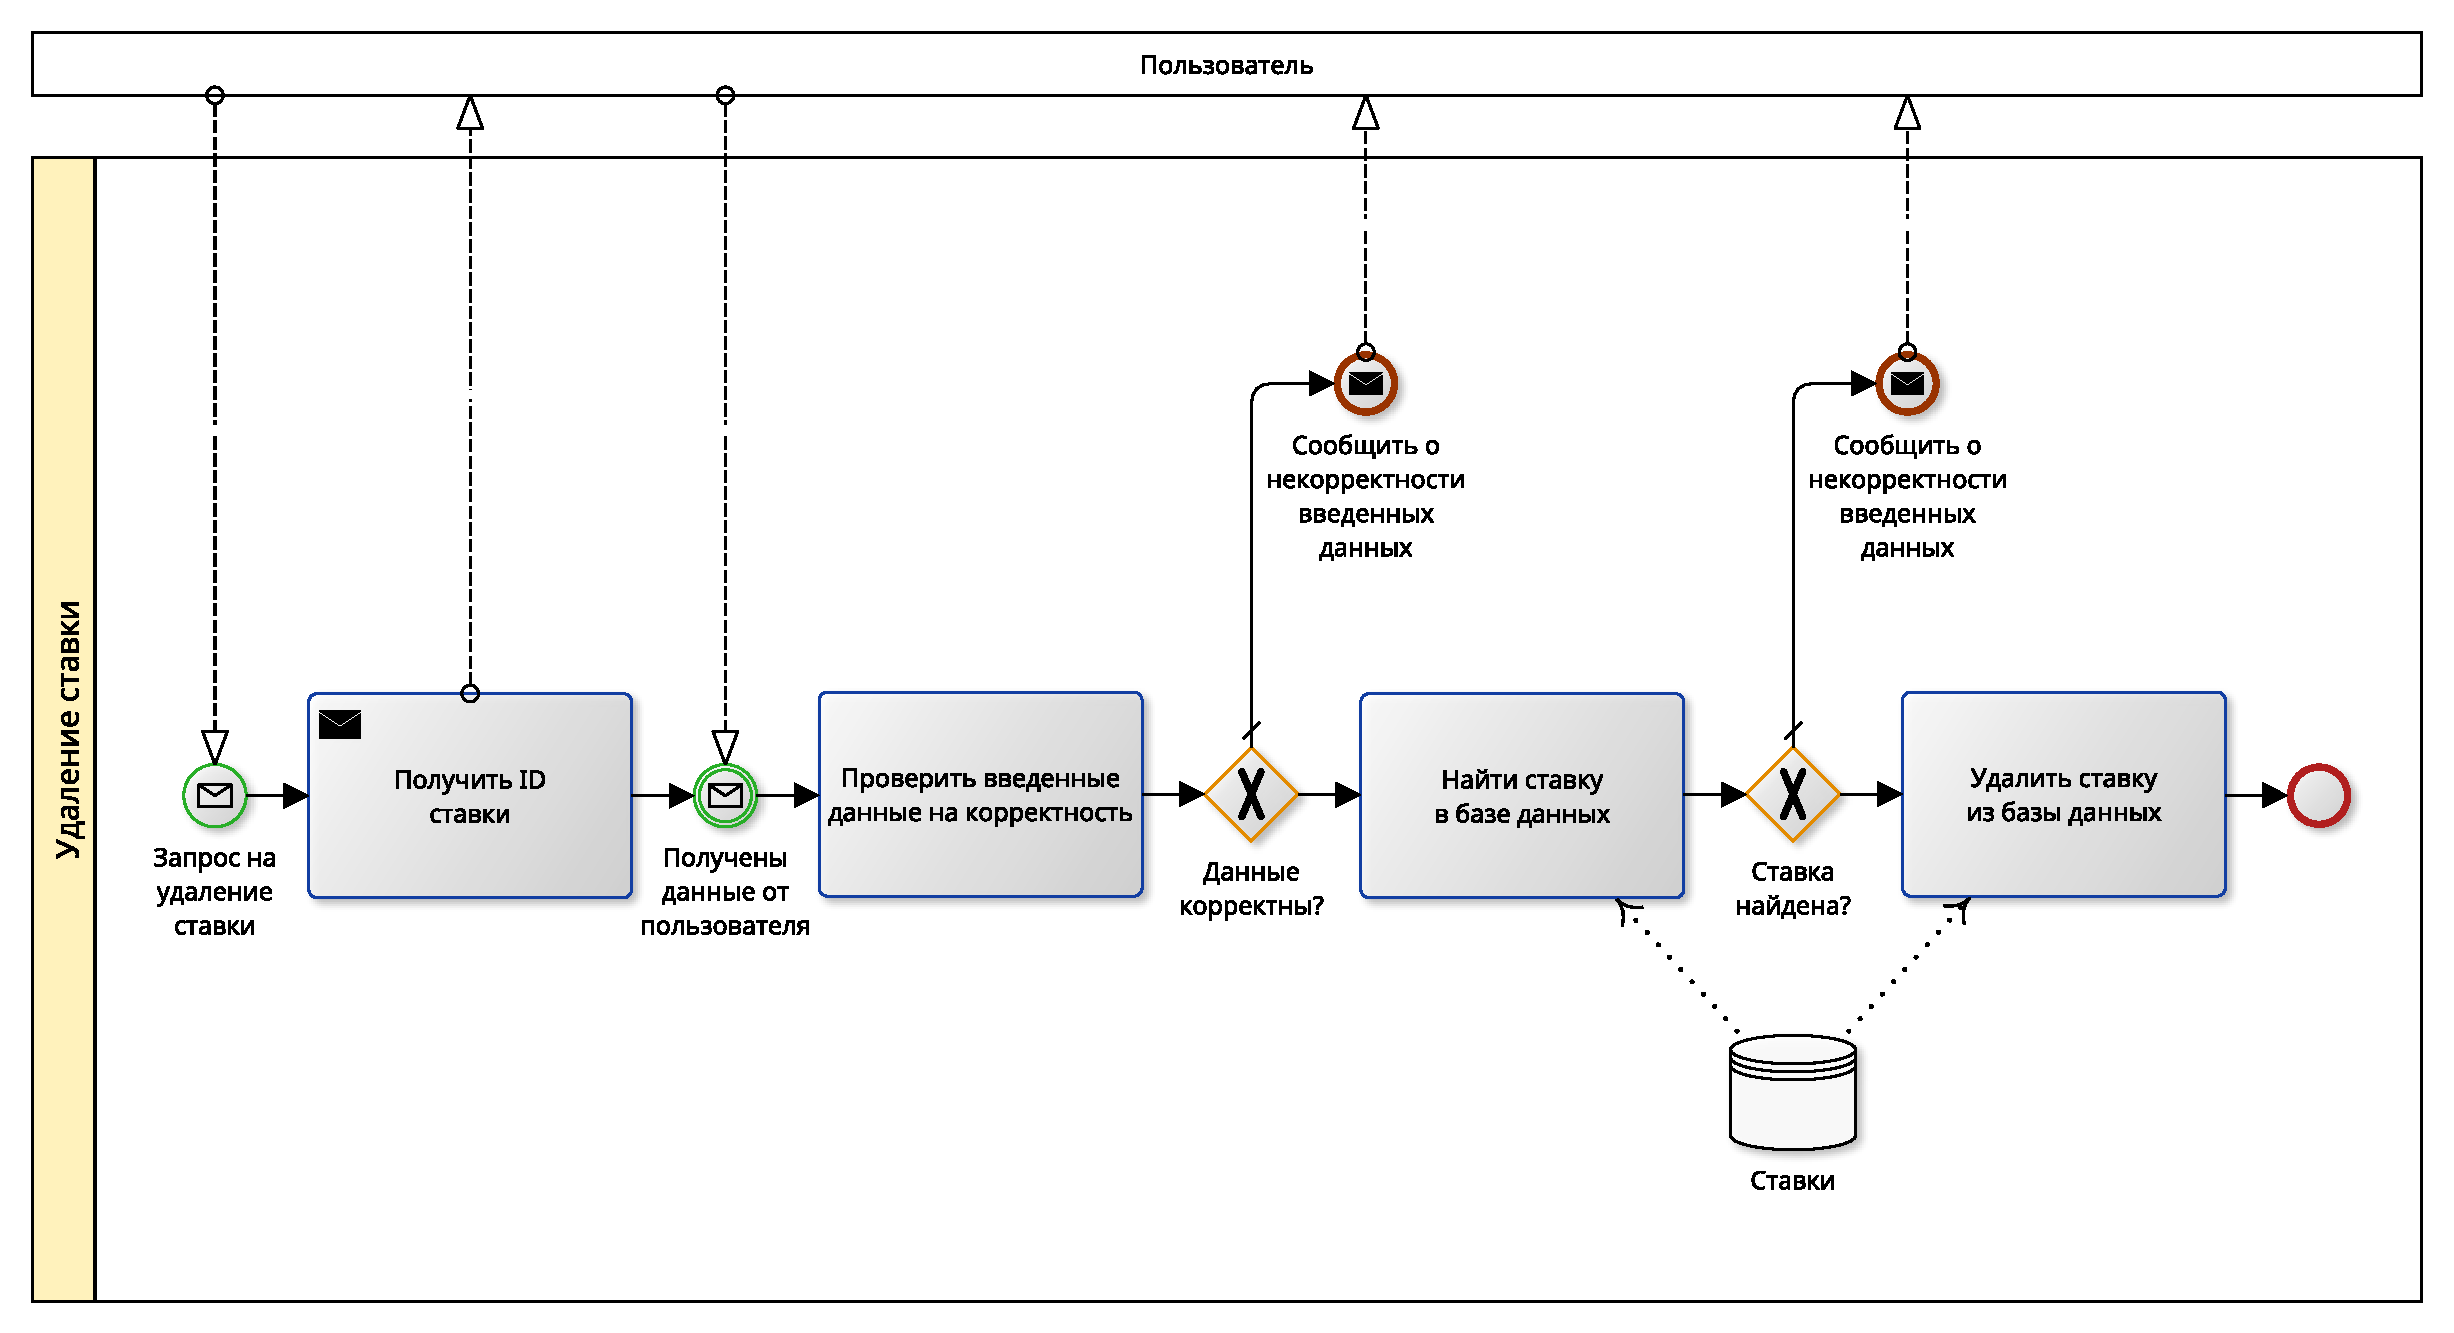
\includegraphics[width=0.8\linewidth]{bpmn_removebet}
	\caption{Бизнес-правило удаления ставки}
	\label{bpmn_removebet}
\end{figure}
\begin{figure}[H]
	\centering
	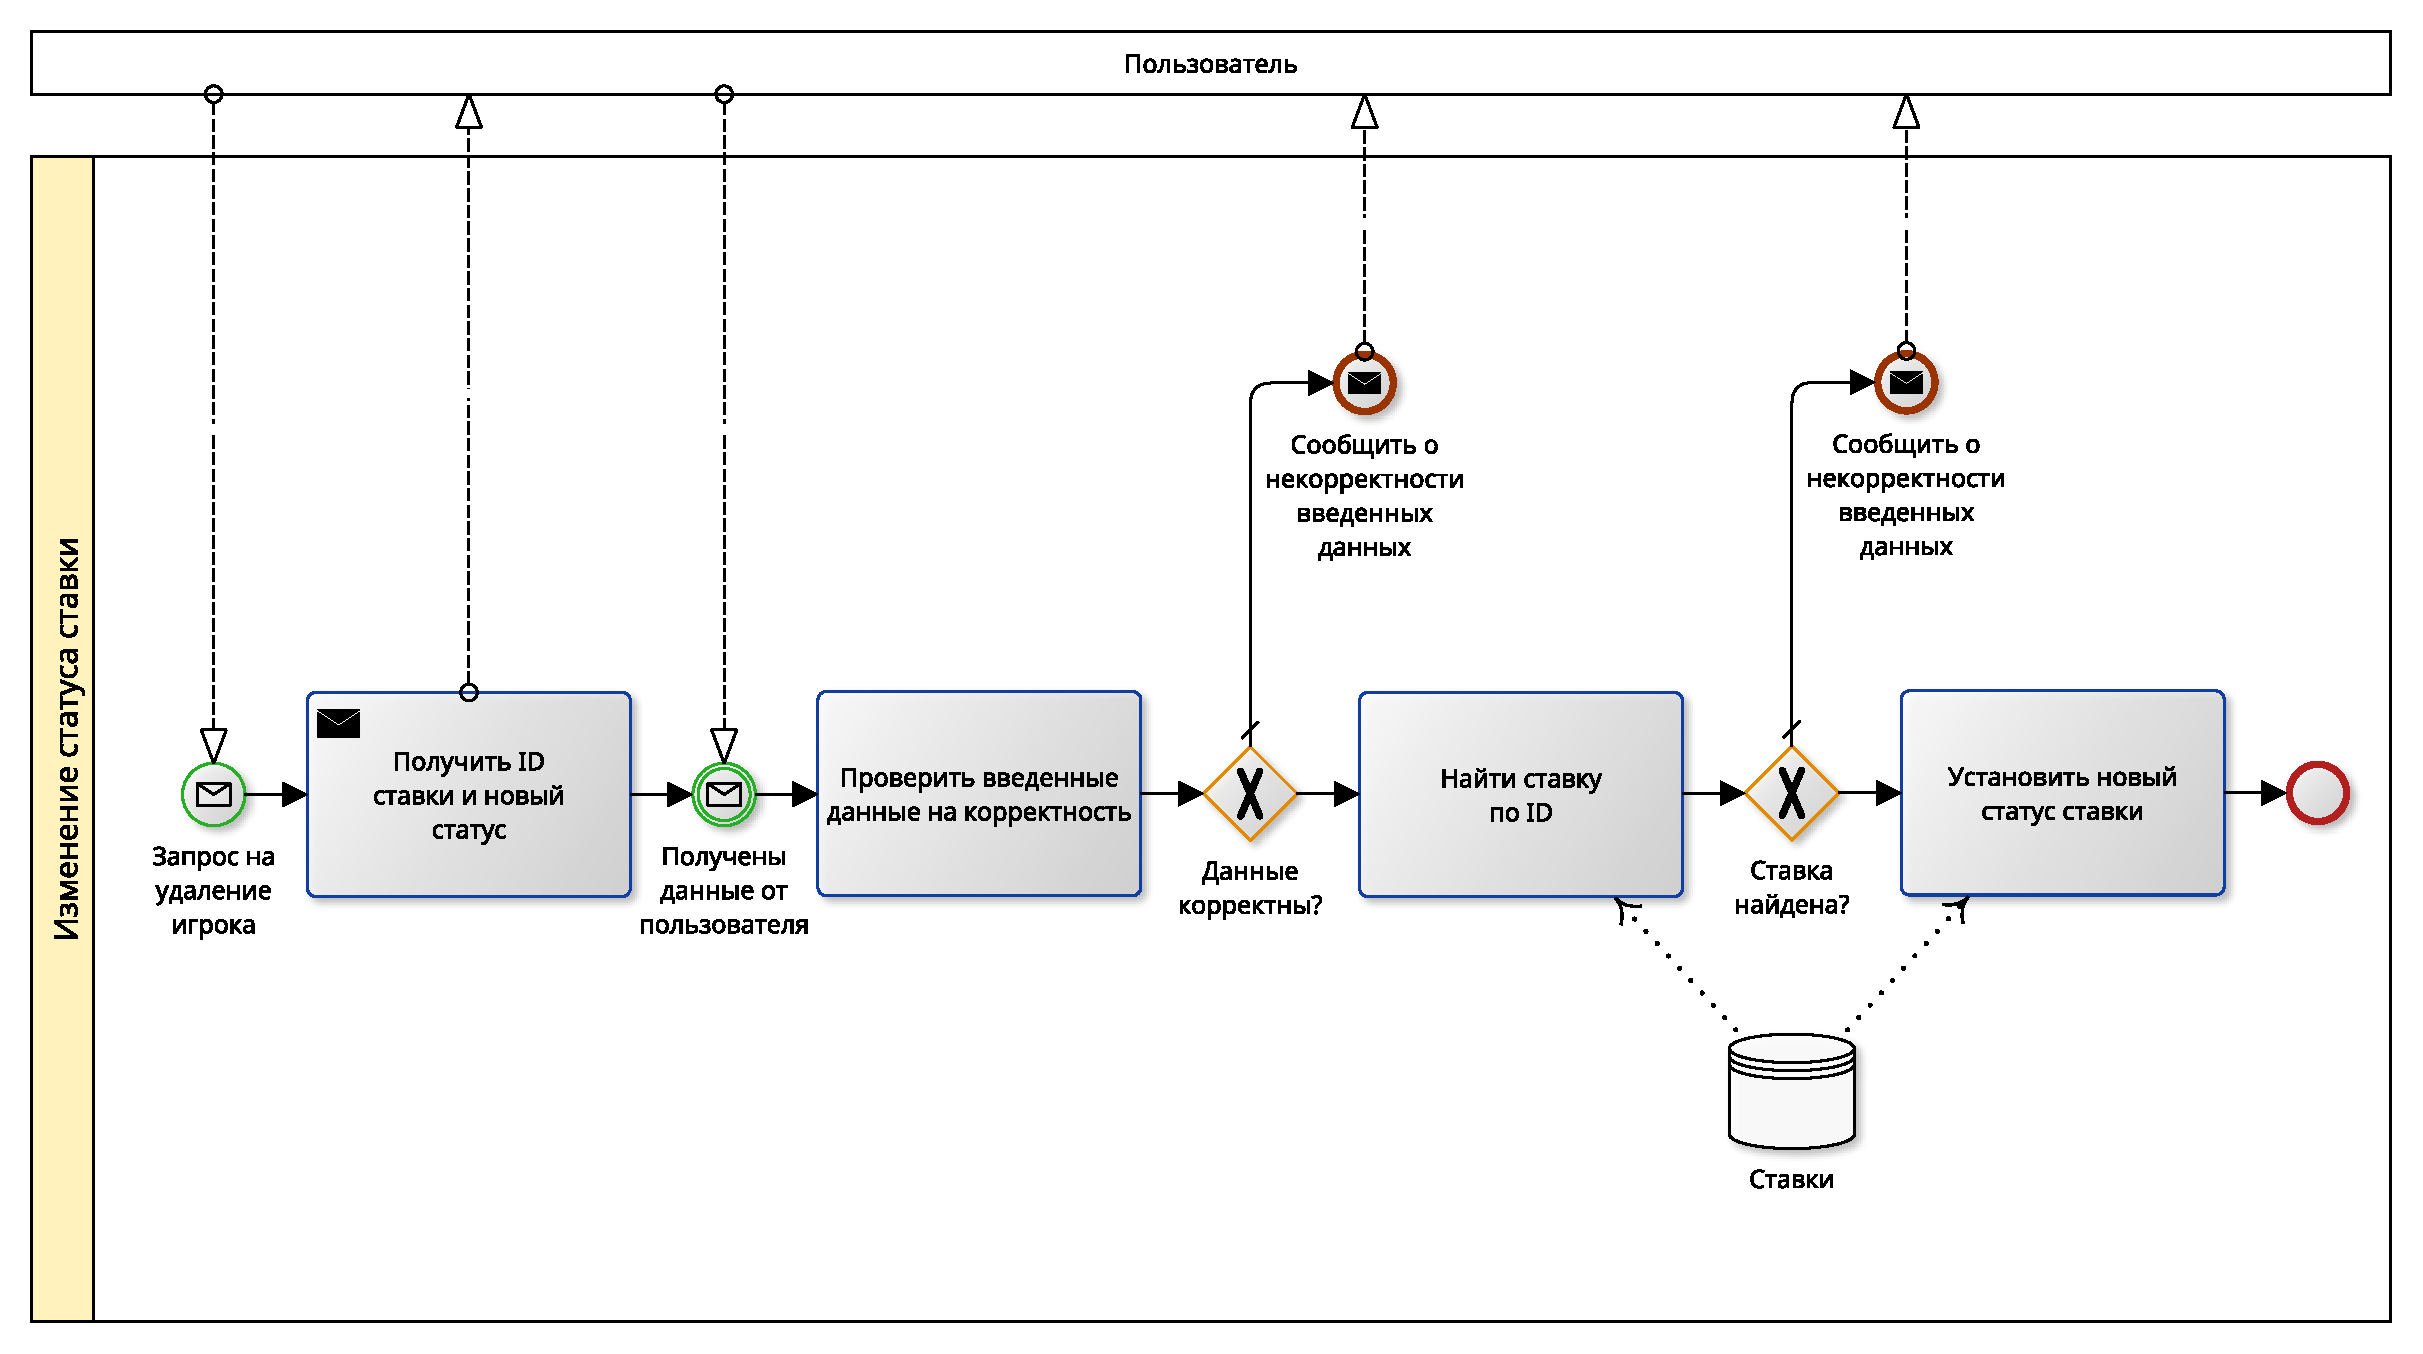
\includegraphics[width=0.8\linewidth]{bpmn_setbetstatus}
	\caption{Бизнес-правило изменения статуса ставки}
	\label{bpmn_setbetstatus}
\end{figure}
\begin{figure}[H]
	\centering
	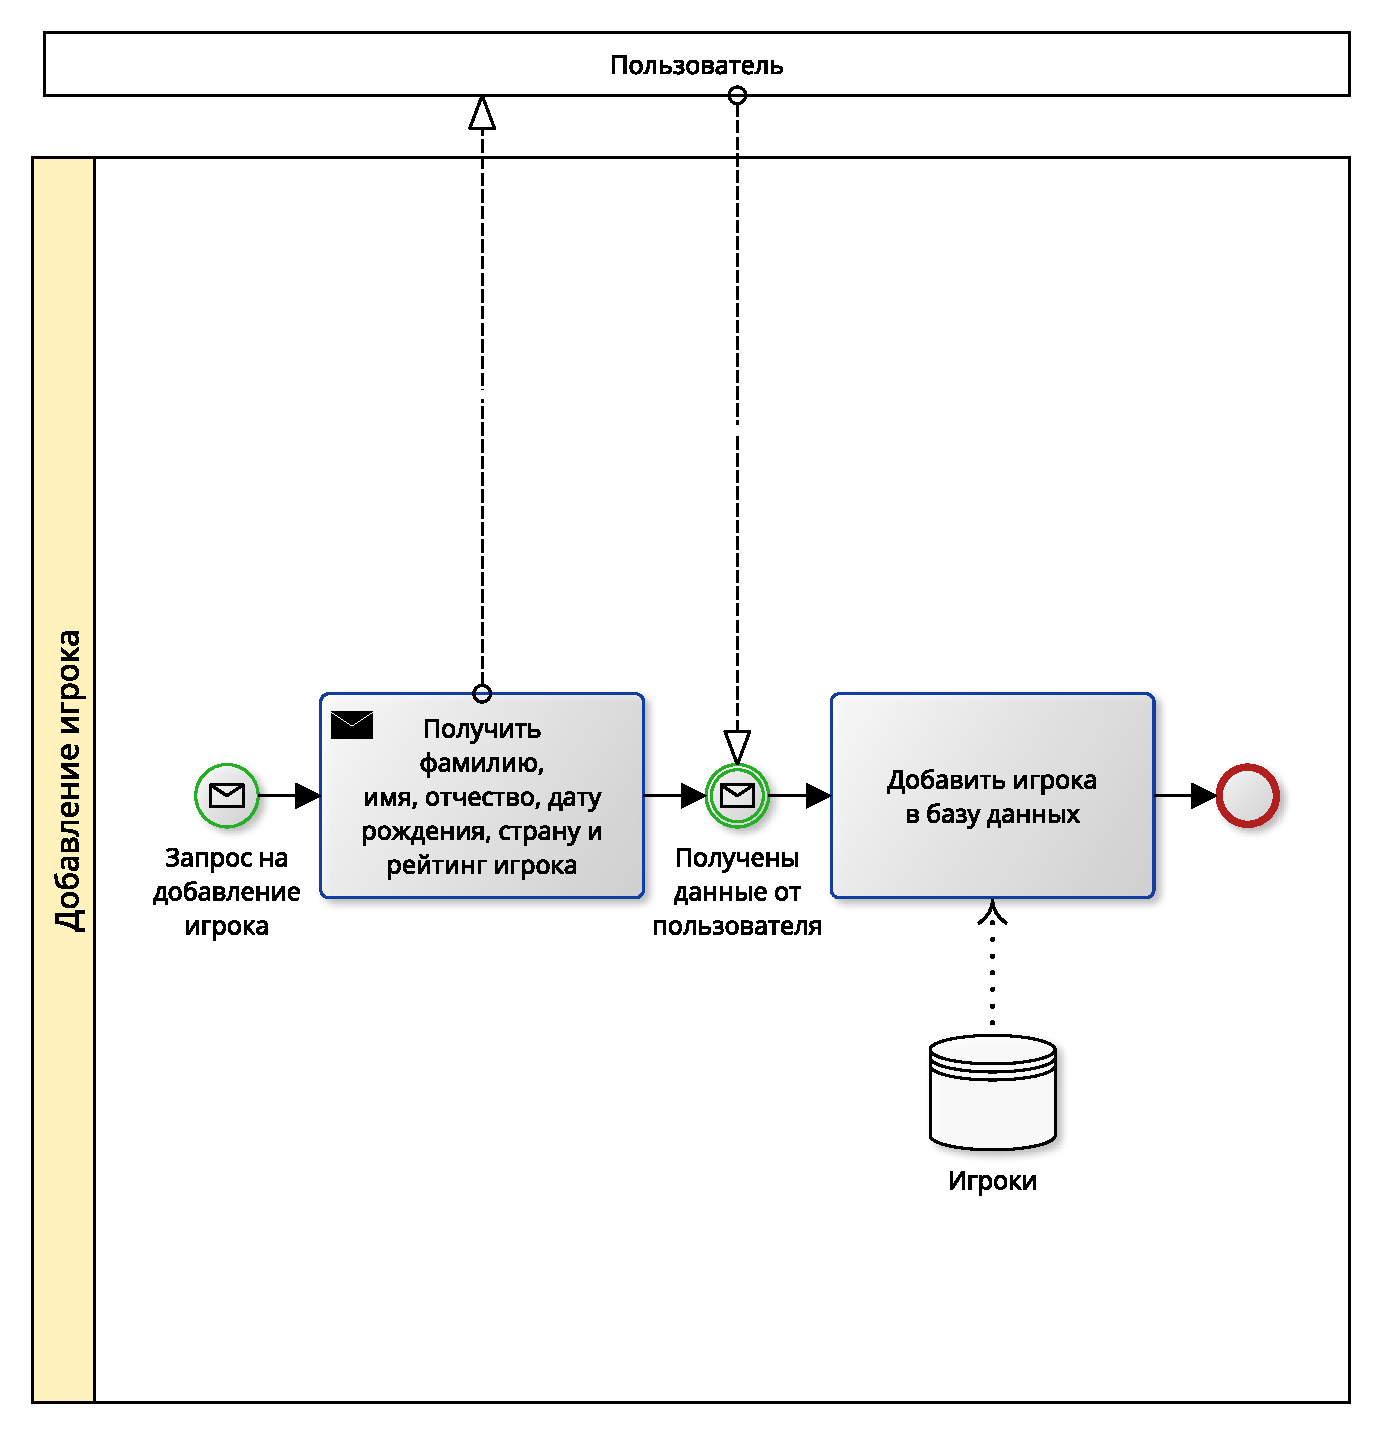
\includegraphics[width=0.6\linewidth]{bpmn_addplayer}
	\caption{Бизнес-правило добавления игрока}
	\label{bpmn_addplayer}
\end{figure}
\begin{figure}[H]
	\centering
	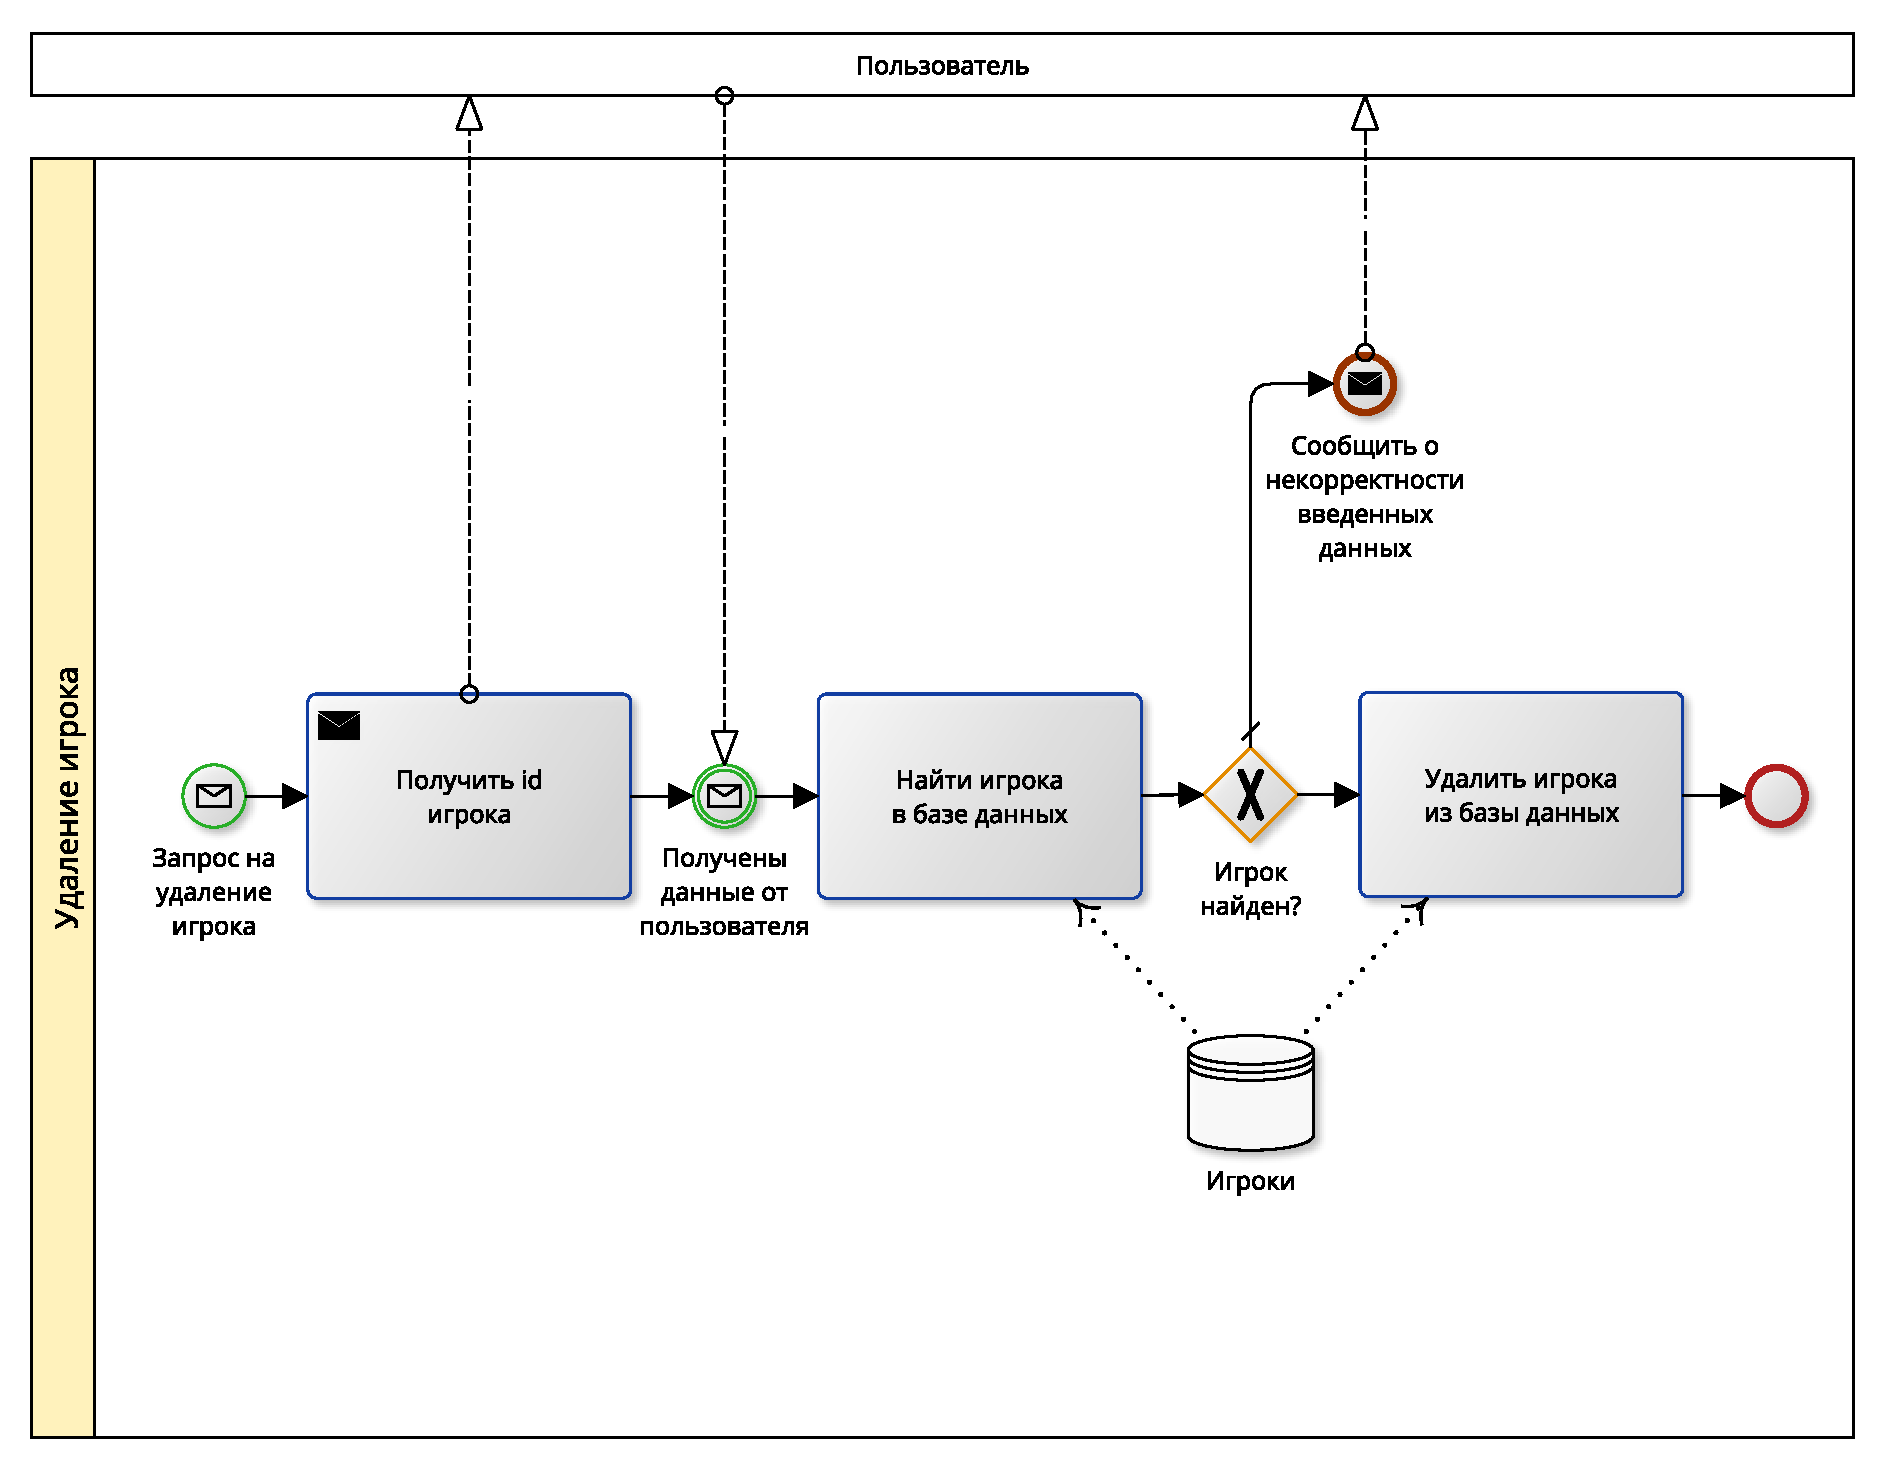
\includegraphics[width=0.8\linewidth]{bpmn_removeplayer}
	\caption{Бизнес-правило удаления игрока}
	\label{bpmn_removeplayer}
\end{figure}
\begin{figure}[H]
	\centering
	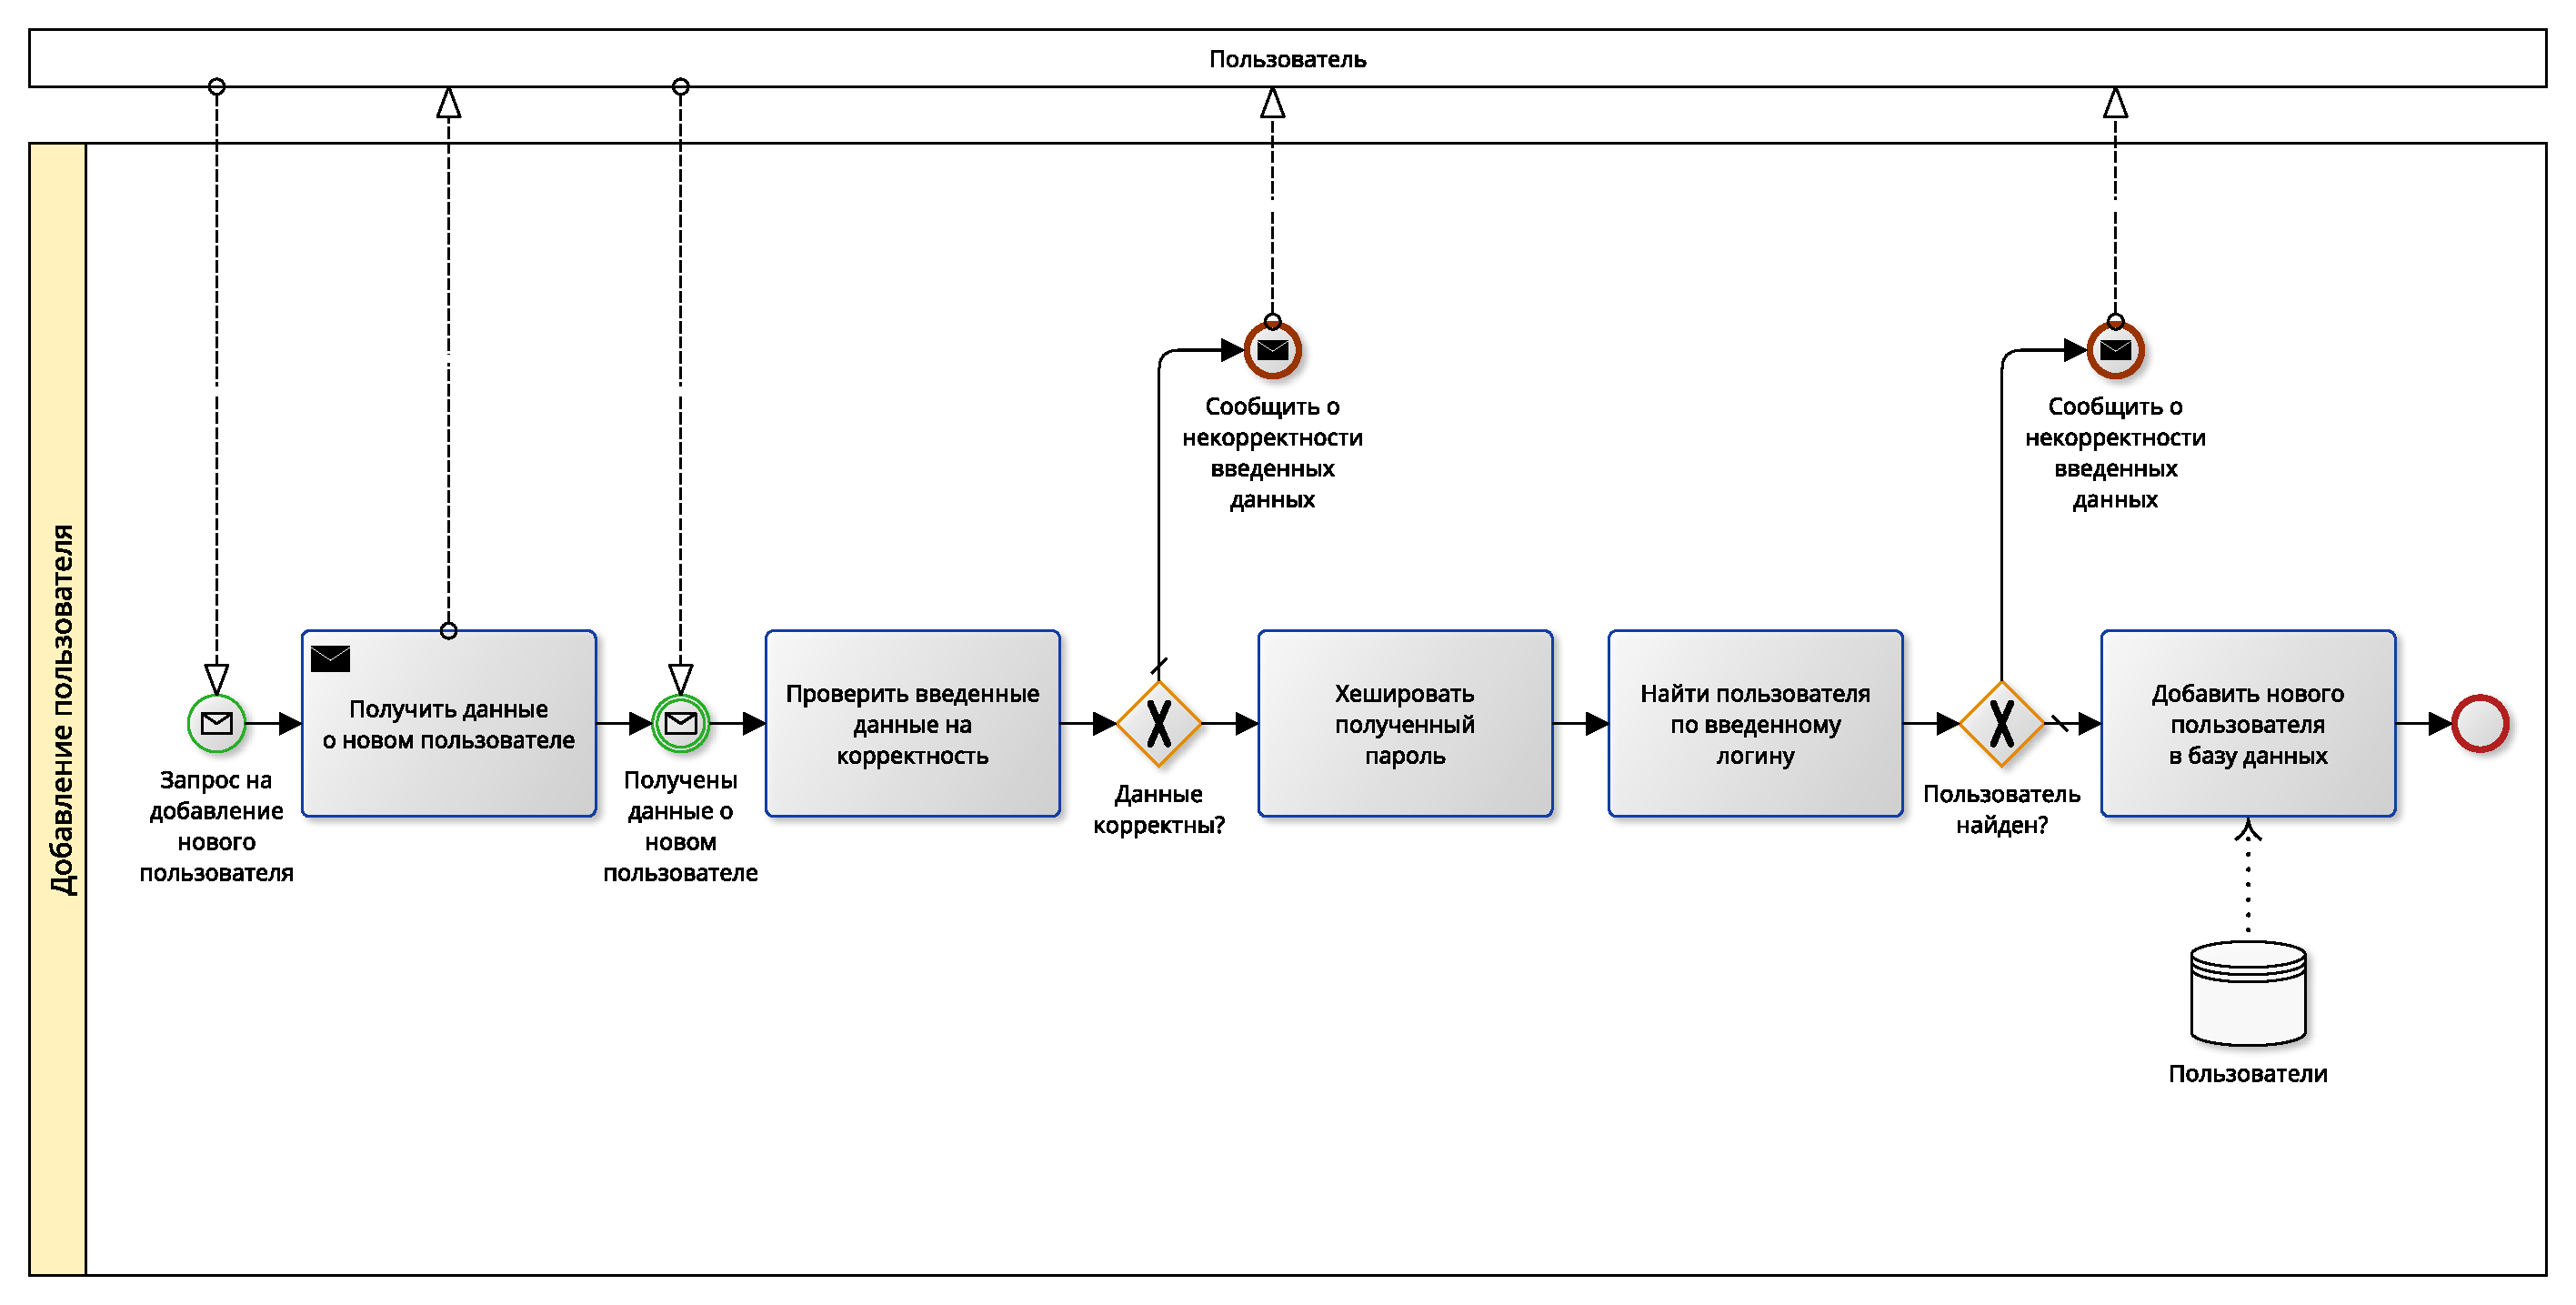
\includegraphics[width=0.8\linewidth]{bpmn_adduser}
	\caption{Бизнес-правило добавления пользователя}
	\label{bpmn_adduser}
\end{figure}
\begin{figure}[H]
	\centering
	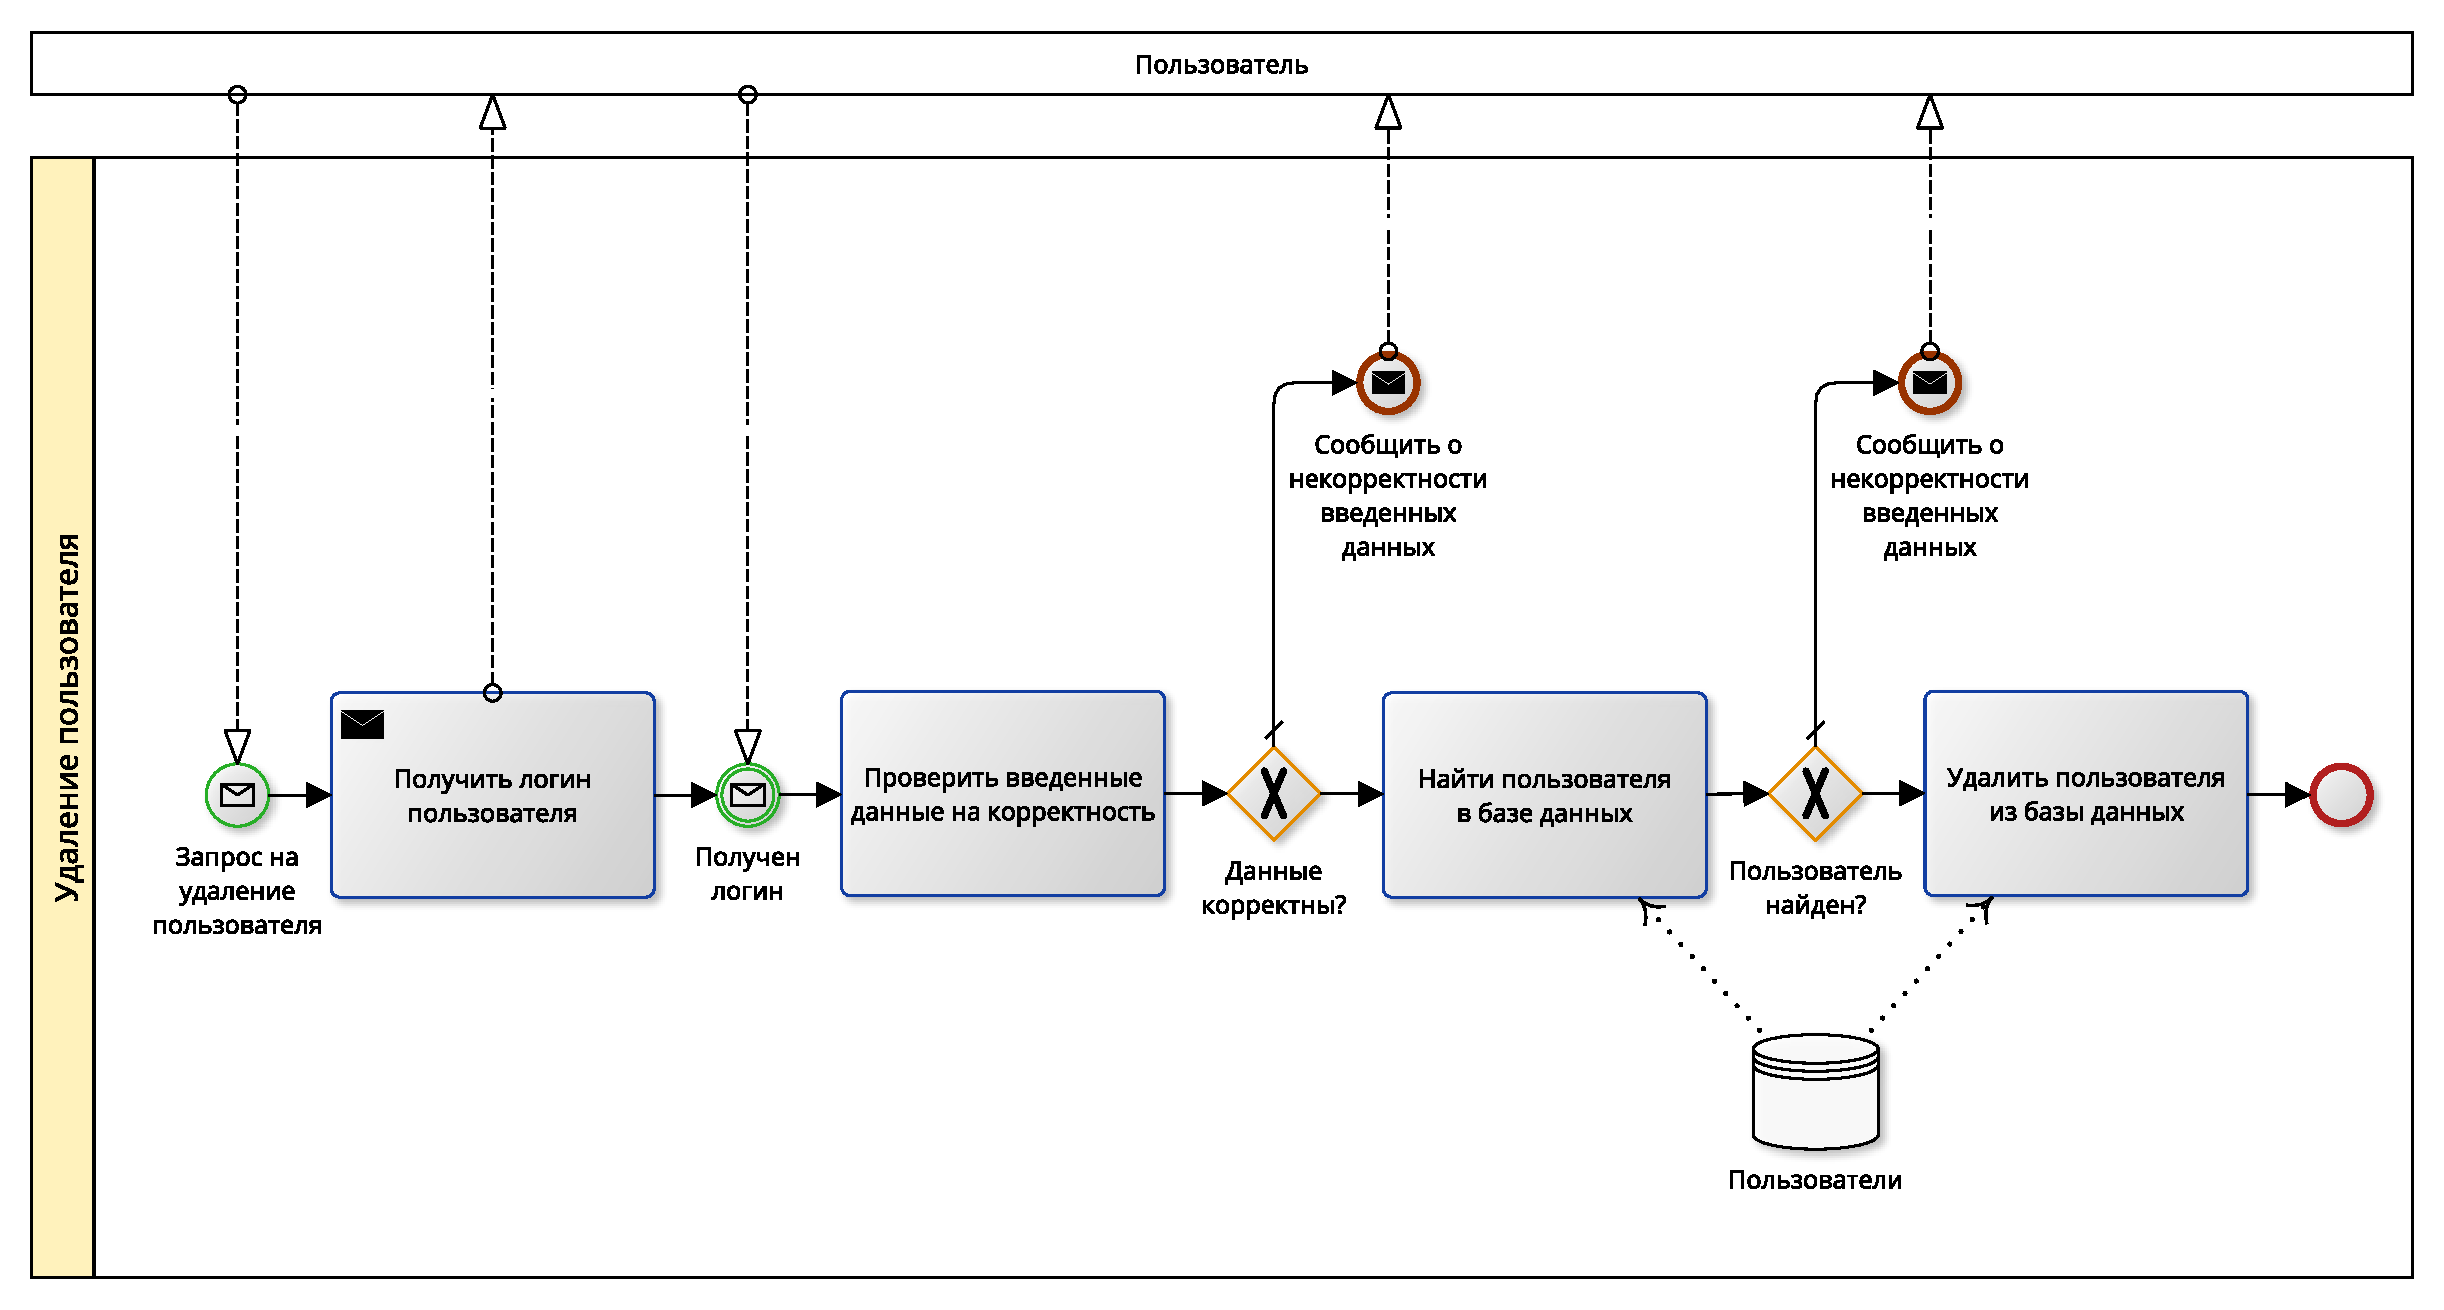
\includegraphics[width=0.8\linewidth]{bpmn_removeuser}
	\caption{Бизнес-правило удаления пользователя}
	\label{bpmn_removeuser}
\end{figure}

\section{Проектирование базы данных}

Из ER-диаграммы предметной области, представленной на рисунке~\ref{er}, следует, что ставка может содержать в себе вложения, которые также являются ставками. Для хранения данных предлагается использовать документоориентированные СУБД, поскольку они ориентированы на работу с иерархическими структурами данных~\cite{docdb}.

ER-диаграмма проектируемой базы данных представлена на рисунке~\ref{dber}.
\begin{figure}[H]
	\centering
	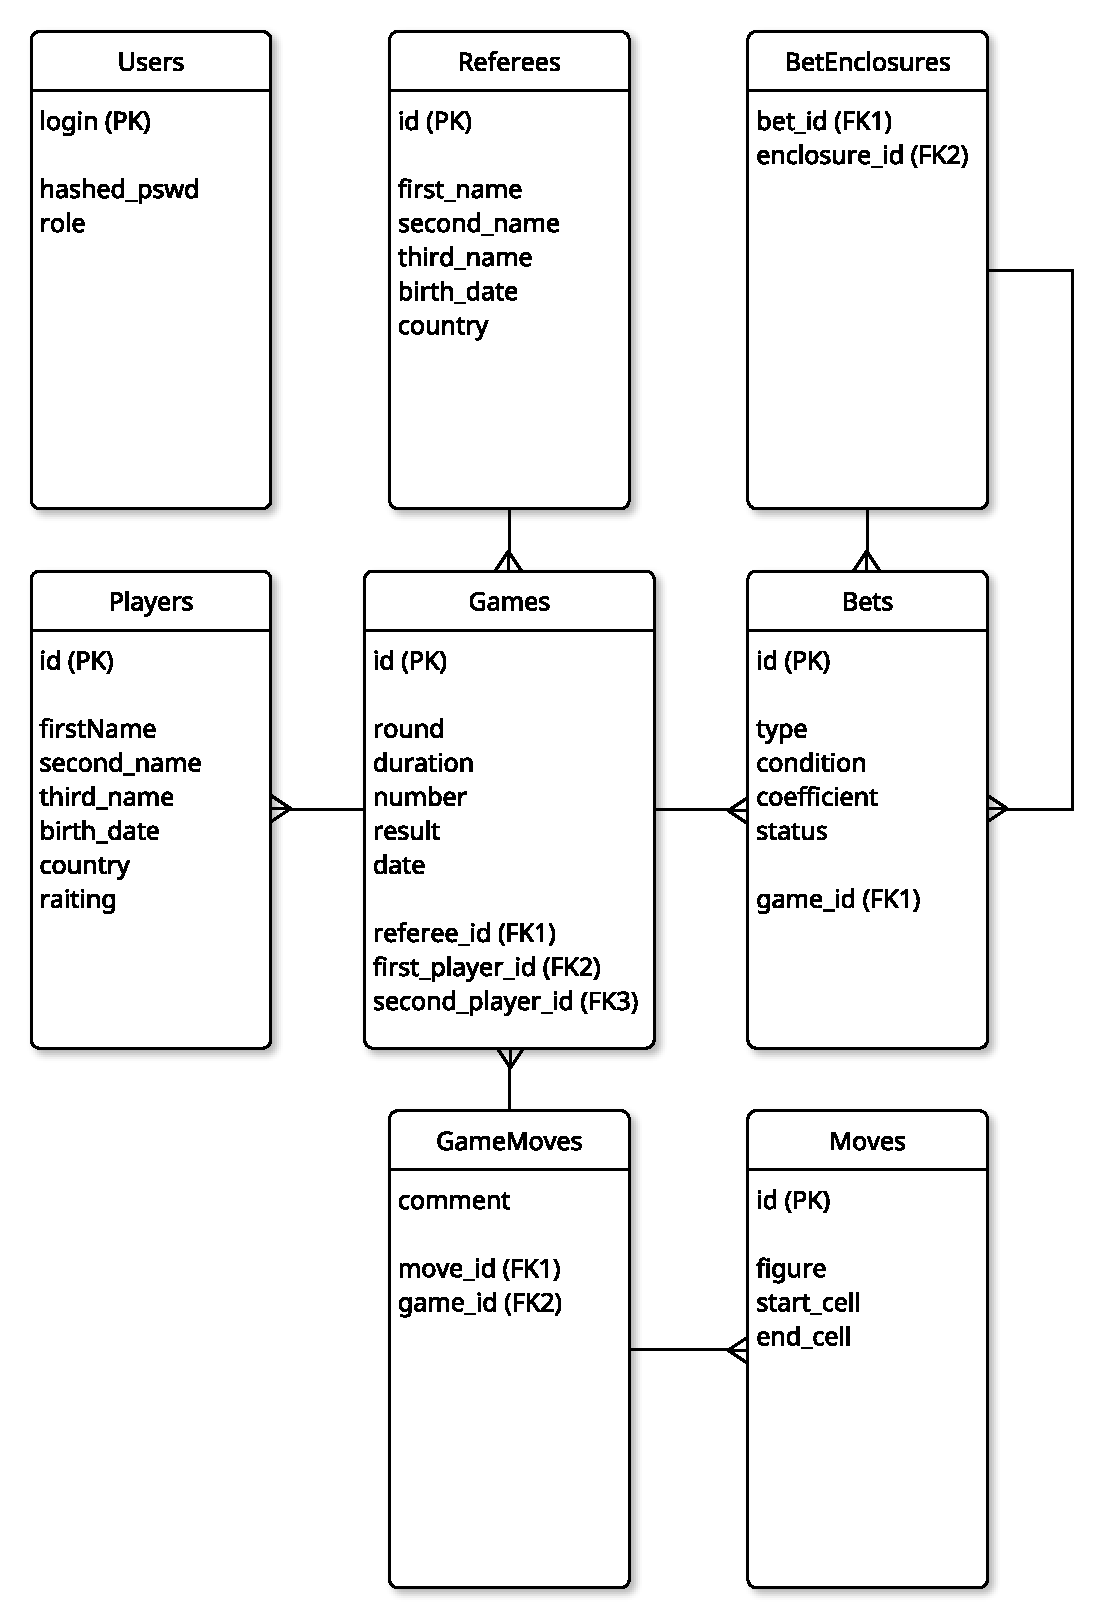
\includegraphics[width=0.6\linewidth]{dber}
	\caption{ER-диаграмма проектируемой базы данных}
	\label{dber}
\end{figure}

Проектируемая база данных содержит в себе следующие сущности:
\begin{itemize}
	\item User~--- информация о пользователях системы;
	\item Game~--- информация о сыгранных шахматных партиях;
	\item Player~--- информация об игроках;
	\item Move~--- информация о ходах, сделанных в партиях;
	\item GameMoves~--- развязочная таблица для установления связи многие-ко-многим между шахматными партиями и ходами;
	\item Bet~--- информация о ставках;
	\item Referee~--- информация о судьях.
\end{itemize}

Для обеспечения целостности проектируемой базы данных вводятся следующие ограничения:
\begin{itemize}
	\item идентификаторы шахматной партии, хода, судьи, игрока и ставки являются натуральными числами;
	\item рейтинг игрока является целым числом;
	\item раунд шахматной партии является натуральным числом, принимающим значения от 1 до 8;
	\item номер матча шахматной партии является натуральным числом;
	\item тип ставки описывается тремя целыми числами~--- 0 (одинарная ставка), 1 (экспресс), 2 (система);
	\item тип фигуры в описании шахматного хода описывается шестью целыми числами:~--- 0 (король), 1 (ферзь), 2 (ладья), 3 (слон), 4 (конь), 5 (пешка);
	\item коэффициент ставки представляет собой вещественное число, большее единицы;
	\item условие ставки является непустой строкой;
	\item статус ставки описывается тремя целыми числами~--- 0 (результата пока нет), 1 (ставка сработала), 2 (ставка не сработала).
\end{itemize}

Для корректной работы с данными необходимо реализовать следующие триггеры:
\begin{itemize}
	\item проверка на выполнение условий ставок (главной линии, экспрессов, содержащих только главные линии; систем, содержащих экспрессы с главными линиями) после добавления завершенной партии в базу данных;
	\item изменение рейтинга игрока после добавления завершенной партии в базу данных;
	\item удаление ходов из шахматной партии;
	\item удаление соответствующих шахматных партий перед удалением игрока из базы данных;
	\item удаление из базы данных ходов, не содержащихся в сохраненных шахматных партий.
\end{itemize}

Схемы алгоритмов триггеров приведены на рисунках~\ref{}--\ref{}.


\clearpage
